
{\centering
\parbox{\textwidth}{%
  \raggedright{

  You can't do inference without making assumptions.\par\bigskip
  }
  \raggedleft\MakeUppercase{A Bayesian friend}\par%
}}

\vspace{5em}

{\centering
\parbox{\textwidth}{%
  \raggedright{

  [We must avoid] false confidence bred from an ignorance of the probabilistic nature of the world, from a desire to see black and white where we should rightly see gray.\par\bigskip
  }
  \raggedleft\MakeUppercase{Immanuel Kant}\\
  \raggedleft\MakeUppercase{AS PARAPHRASED BY MARIA KONNIKOVA}
  \par%
}}

\chapter{Probabilistic modelling}\label{ch:02}

\begin{chapter_outline}

  % The previous chapter established that modelling has played a major role in the progress of science and engineering.
  In this chapter, we argue that accounting for uncertainty is crucial for building useful models, and we present a background on the \textit{probabilistic modelling} framework.
  More precisely, this chapter shall answer the following questions:
  \begin{enumerate}
    \item What is a probabilistic model?
    \item How do we build a probabilistic model?
    \item How can we use a probabilistic model?
    \item What are the technical challenges considered in this thesis?
  \end{enumerate}
    For this purpose, we start by abstracting the main concepts orbiting around probabilistic modelling. We motivate the relevance of developing powerful tools in this context and we provide an overview of two classes of models relevant to this thesis, probabilistic graphical models and deep probabilistic models.
% This chapter concerns the definition of unsupervised learning with a brief review of classical methods.
% Graphical models (in particular B-net are introduced here.)
% It continues with a review of deep generative modelling, with a discussion between explicit and implicit generative modelling.
% We introduce the concepts of GANs, Energy based models, VAEs, Normalizing Flows and diffusion models. With a note that VAEs and diffusions models
% are discussed in more details in further chapters.
\end{chapter_outline}

% \textcolor{red}{Clearly mention that deep generative models is a class of probabilistic model and so it is important to first clarify what are probabilistic models; why they are useful and why this is still q very qctive reserch area. (it might be simple to add this in the outline.)}

\section{Introduction}
The invention of computers has enabled the automatisation of many tasks historically accomplished by humans. One key ingredient of this revolution is making computers \textit{reason} - to make an informed judgment based on logical arguments and observations. The set of hypotheses on which this logic builds is a \textit{model}. Both humans and machines rely on reasoning to perform tasks. As an example, let us consider that we want to choose a bottle of wine at the restaurant. We first need some hypotheses, e.g., - What kind of wine do people like at the table? Red or white? Strong or delicate? - What is the budget? - What do we have on the menu? - What is the wine list? Etc. Provided with this model, we can make an informed choice: remove the wines that are too expensive or would unplease someone at the table, and pick one of the remaining that goes well with tonight's dinner? Other examples include a scientist who needs a model of the earth and its atmosphere to explain climate change; or streaming platforms which use a model that represents users' tastes to make video recommendations.

In these contexts and many others, the model plays a central part. In practice, we aim for \textbf{faithful models} - models for which reasoning leads to a proper judgment. In the examples mentioned above, we strive for models that help us choose the right wine; that explain the climate over the last centuries; that keep the user longer on the platform. The exact definition of the model's quality depends on the targetted application. However, certain classes of models are usually strictly better than others.
In particular, a model that embeds notions of uncertainty is more expressive than the deterministic version. Deterministic models do not accurately represent phenomena that exhibit randomness. Although it is unknown whether the laws that rule our reality are deterministic or stochastic, modelling requires simplifying assumptions which induce stochasticity. For example, a model that acknowledges partial observability of a sytem needs to express its uncertainty about the state of these unobserved variables. Uncertainty may also arise from the finite precision of measurement devices or from simplifying approximations that cannot make perfect predictions.

We thus need a language to formally express this stochasticity. The language of \textit{probability} is the one to make statements about uncertain events. It allows contrast between what is \textit{possible} and what is \textit{plausible}. The distinction is essential as it will enable us to eventually make deterministic decisions by focusing on the most plausible events and discarding other events which are unlikely. For example, wine amateurs know that an old bottle has a higher chance of being corked than a recent one but might also taste better. We can use probability to express this fact and select a bottle to our taste with high probability.

\subsection{Probabilistic model}
A probabilistic model is a model that describes a phenomenon of interest in probabilistic terms. Practically, it defines a probability distribution over the set of variables considered valuable to describe the phenomenon (e.g., $X, Y, Z$). When it models the joint observations, the distribution can be the joint between all variables (e.g., $P(X, Y, Z)$). It can also be a conditional distribution  (e.g., $P(X \mid Y, Z)$) if some of the variables are known when using the model. We mostly limit our discussion to the former case for simplicity but with no loss of generality.

\begin{side_note}{Formalism}
  In this background, we will abstract the domain (discrete or continuous) of the random variables when possible. The term (conditional) probability distribution refers to the object $P$ that fully describes the stochastic behaviour of a random variable $X$ taking values in $\mathcal{X}$. When the domain $\mathcal{X}$ is discrete, $P$ corresponds to the probability function $P(X=\cdot): \mathcal{X} \rightarrow \left[0, 1 \right]$ that satisfies the three Kolmogorov's axioms. In the case of a continuous domain, we will narrow our discussion to real values $\mathcal{X} \triangleq \mathbb{R}^d$, where $d$ is the dimensionality of the random variable. In this context, the probability distribution is the density function $P(X=\cdot): \mathcal{X} \rightarrow \mathbb{R}_{+}$ which defines the probability that a realization $\bm{x}$ of $X$ lies in a sub-domain $\mathcal{A}$ as $\int_{\bm{x} \in \mathcal{A}} P(X=\bm{x}) \text{d} \bm{x}$. The probability functions implied by the density must also satisfy Kolmogorov's axioms. In this chapter, we clearly mention the domain of the random variable when it matters for the discussion. In the next chapters, we will focus on the continuous case, hence we will use the standard notation $p$ to denote the probability density function.
\end{side_note}
% For discrete variables, the mathematical object $P(X, Y, Z)$ is a probability and a density for continuous variables. In the following of this chapter, we will often use the symbol $P$ with no additional mention of the variable's type (discrete vs continuous) to generalise the discussion to both types.

One goal of building a probabilistic model, arguably the main, is to perform \textit{inference}. That is to answer questions in the context of a model, to reason. These questions come in different flavours. What is the most likely value of $Y$ if we are to observe $X$? What is the conditional distribution of $Y$ in this case? It is also different whether we want to evaluate the value $P(Y \mid X)$ or just sample from it. For these purposes, the probabilistic models may have to handle different queries: \textit{marginalisation, conditioning, sampling, and probability evaluation}.

Certain representations are appropriate for a subset of queries and not for others. For example, we can represent the discrete distribution between $X, Y, Z$ with a $3$D table where each entry stores the corresponding joint probability. The evaluation of the joint probability is very efficient with this representation. However, evaluating a conditional distribution requires going over each entry corresponding to the conditioning value and re-normalising the probabilities by their sum. Sampling, as well as marginalization and conditioning, becomes very inefficient as the number of entries in the table grows. And the number of entries grows exponentially with the number of dimensions. Fortunately, there exist alternative representations such as the one we review below.

The following sections provide an overview of two main classes of probabilistic models, namely \textbf{probablistic graphical models}~(PGMs) and \textbf{deep probabilistic models}~(DPMs). As its name says, the former class aims for a graphical representation of the distribution. It allows understanding the modelling assumptions, such as independence hypotheses, quickly. The latter focuses on models whose internal representations use deep neural networks. Some of these models are especially well suited for sampling and are often called \textbf{deep generative models} in this case. We discuss the particularities of each class of models and provide a thorough description of the main algorithms that perform the different queries aforementioned.

In this manuscript, we argue on multiple occasions that we shall not make a rigid distinction between graphical and deep generative models as they are just different representations of the same mathematical object. Some deep probabilistic models have a direct correspondence within the graphical family, enabling abstract reasoning independent of the neural network architectures. However, for clarity, we will first introduce probabilistic graphical models. And then borrow the newly introduced notations and concepts to describe several deep probabilistic models.


\begin{side_note}{Bayesian vs frequentist interpretation}
  Two interpretations of probabilities compete with each other. In the above discussion, we brought probabilities as a language to express our uncertainty about the truth of facts. We took the \textit{Bayesian} interpretation of probabilities. The reference to sir Bayes comes from the application of Bayes' rule to update our prior belief in the presence of new evidence. In this context, the prior is part of the model and affects its quality. The main drawback of the Bayesian interpretation is the potential complexity of defining the prior appropriately. The other view, referred to as \textit{frequentist}, interprets a probability as a frequency of events. With this perspective, probability does not quantify uncertainty; it expresses intrinsic randomness. Frequentists reject the notion of prior belief, which has pros and cons. In general, there is no interpretation better than the other. However, the Bayesian interpretation provides motivations for many popular algorithms in machine learning and is the one we will often implicitly use in our discussions. At the same time, we do not strictly reject the frequentist point of view. For example, we discuss the maximum likelihood principle, a frequentist concept.
\end{side_note}
% Now contrast between discriminative versus descriptive models.
%
% Say that what differentiate models is the intrinsic distribution modeled but also in practice the exact way the distribution is expressed is important (reference to implicit versus explicit).

\subsection{Learning}
% Before jumping into the description of different classes of models, we can keep our discussion generic longer.
Until now, we have implicitly assumed the model was given to us. However, this is not realistic in many settings. For example, how can I accurately model my wine taste? Ranking all world's wines is not an option. It might be too expensive and would not help me finish this dissertation. However, I could answer a list of questions and then figure out a summary of my tastes for the principal characteristics of wine. The task of summarising my answers is \textit{learning} - to build a compressed representation of observations (my answers). Afterwards, we can use this representation to perform an informed guess. This representation is a model, a simplified representation, of my wine taste. Learning is thus the task of instantiating a model from data.

In practice, we do not perform \textit{learning} without additional assumptions. Instead, we define a set of models among which we believe at least one would be a good representation of the phenomenon of interest. If we are Bayesians, we even add a probability that summarises whether or not we believe the model is good. We will come back to the Bayesian prospect later but for now, let us assume we do not have any a priori of the models' quality.

The class of possible models can be finite, e.g. the class contains two models - one for people who like red wine and white wine; the other for people who only like red wine. Compressing my taste into one of these models goes with a significant loss of information but might already be helpful in some settings. The class of models can be infinite, e.g. if parameterised by real values. For example, we can summarise wine taste by attributing an affinity score to each of the main features of wine.
\paragraph{Maximum likelihood estimation.}
A learning strategy is a set of rules that produces a model from data. When we only consider a finite number of models, a simple strategy exists. We test the predictive performance of each model and select the one that is the most consistent with our data. If the models describe the phenomenon with discrete events, we maximise the probability. If it considers a continuous set of events, we maximise the density. In the case where one of the models is \textit{correct} - it is the one that generates the data - this selection algorithm will eventually select the right model as the number of independently and identically distributed (iid) data points tends to $\infty$. This selection technique is said \textit{consistent}.

We can use a similar approach when the models are parameterized by a real vector $\bm{\theta}$. In this case, our goal is to estimate a good value for $\bm{\theta}$. One approach, denoted maximum likelihood estimation (MLE), is to select the model's parameter $\bm{\theta}$ that maximizes the  joint distribution (density or probability) of the data $\mathcal{D}$. This quantity is called the likelihood function of the parameter $\bm{\theta}$, denoted $\mathcal{L}(\bm{\theta}) \triangleq P(\mathcal{D}\mid\bm{\theta})$. Hence the MLE estimator is formally defined as
\begin{align}
   \bm{\theta}_{\text{MLE}} = \argmax_{\bm{\theta}} P(\mathcal{D}\mid\bm{\theta}). \label{eq:chap02:MLE}
\end{align}
In the presence of iid data, this estimator is consistent - provided a class of models that contains the `true` generative process, it eventually recovers the `true` model as the number of points tends to $\infty$. Formally, the consistency property is a convergence in probability of the estimator to the exact value, and it requires additional assumptions that ensure the model is identifiable and the likelihood function is well behaved. %(compactness and continuity to $\bm{\theta}$, and dominance)

The consistency of the MLE is an appealing property. However, we must consider the central assumption it relies on very carefully! While ensuring that the model class contains the true generative process is ok in artificial settings. For real data, this assumption is a metaphysical question. The law of large numbers saves us if we only look at things on average and are provided with many data, but it does not apply to all modelling tasks. Sometimes, we know this assumption does not hold, but we would still like to learn a good model; the MLE principle does not say much. Even if we know the model class contains the correct model (e.g., if we consider a parametric universal density approximator), the convergence speed with respect to the dataset size is unknown. Moreover, the optimisation of \Cref{eq:chap02:MLE} is often non-trivial.


\paragraph{Learning as inference.}
The strict delimitation between possible and impossible models is another limitation of the MLE approach. Instead of interpreting learning as model selection, we can reformulate learning as an inference task to alleviate this limitation. In this context, the model is a generic description of the phenomenon parameterised by some explanatory variables. For example, the model can be a parametric function, exactly as when we define a class of models in the MLE approach. The distinction between learning as inference and MLE lies in our interpretation of the parameters. In the former, we consider the parameter $\bm \theta$ as part of the model rather than defining a class of models. The MLE is usually associated with a frequentist interpretation of probability, whereas learning as inference is Bayesian.

Let us say we want to learn a model that can predict the conditional distribution $P(Y=y\mid X=\bm{ x})$ that I like a wine with features $\bm{ x} \in \mathbb{R}^d$, where $y \in \mathbb{R}$ is a value that represents my affinity with the wine. Learning aims at summarising the information in the data to perform the task of interest, that is, to predict $P(Y \mid X, \mathcal{D})$.

We parameterise the class of models with a neural network $\bm{ x}$, $f_{\bm \theta}(\cdot; \bm{ x}): \mathbb{R} \times \mathbb{R}^{d} \rightarrow \mathbb{R}^+$, parameterised by $\bm{\theta}$, and which defines a parametric density function over $\mathbb{R}$ conditioned on an input $\bm{x}$. Said otherwise, $f_{\bm{\theta}}$ represents the conditional distribution $P(Y \mid X, \bm{\theta})$. We assume the parameters $\bm{\theta}$ are expressive enough to summarize all information about the ``true'' distribution $P(Y\mid X)$ contained in the data $\mathcal{D}$, that is $ Y \indep \mathcal{D} \mid X, \bm \theta$. Then learning requires 1) to condition our predictions on the data $\mathcal{D}$ and; 2) to marginalize with respect to the unknown value of parameters $\bm \theta$. Taking advantage of the conditional independence $ Y \indep \mathcal{D} \mid X, \bm \theta$, the model for making new predictions is expressed as
\begin{align}
  P(Y=y\mid X=\bm x, \mathcal{D}) &= \int P(Y=y\mid X=\bm x, \bm \theta) P(\bm \theta \mid \mathcal{D}) \text{d}\bm{\theta}\\
  &=\int f_{\bm \theta}(y; \bm x) P(\bm \theta \mid  \mathcal{D}) \text{d}\bm{\theta}.
\end{align}
The data are only used through the posterior distribution $P(\bm \theta  \mid  \mathcal{D})$, representing our updated belief about the best models in light of the observed data. Learning thus amounts to compute $P(\bm \theta \mid \mathcal{D})$, which is an inference task.

We have presented Bayesian inference in parametric spaces; however, these concepts generalise to functional spaces. In this context, we need to define a prior distribution over functions (e.g., L2 integrable functions) and be able to evaluate the likelihood defined by each function. This is usually handled by kernel methods such as Gaussian processes and will not be discussed in this thesis.

Keeping track of the complete posterior distribution can be cumbersome in practice. We can avoid this by selecting the maximum a posteriori (MAP) sub-model. In the case of a parametric model this means freezing the parameter $\bm \theta$ to their most plausible value $\bm \theta_{MAP} = \argmax_{\bm \theta} P(\bm \theta \mid \mathcal{D})$.

Learning as inference strictly generalises the MLE principle to settings where the prior knowledge is more subtle than a binary choice between possible and impossible models. If the prior is non-informative, i.e. the prior does not attribute more credibility to one value of parameters than another, the method is equivalent to the MLE. And when we have prior knowledge, this strategy naturally reduces the importance of unlikely model instantiations and prefers models that are the most plausible given the data and our prior beliefs. Moreover, the MAP is also consistent; it eventually selects the `right` model instance.

% Learning as inference is sometimes criticised by practitioners who do not like the concept of attributing plausibility to the different instantiations of the model. However,
The advantage of the Bayesian learning paradigm is to force the explicit formalisation of modelling assumptions and the prior knowledge associated with each learnable component of the model. It acknowledges that learning a model is a subjective task. Occam's razor says we should always favour the simplest of potential explanations. The Bayesian approach may naturally handle this principle by attributing higher plausibility to simpler model instantiations. This is not true for the MLE approach, which requires ad-hoc algorithms or regularisation objectives to favour simpler models.

% Say that the joint distribution defined by the probabilistic is sometimes learned conditionaly to an input x, without caring about modelling the distribution over x. This is what is called supervised learning. Usually contrasted with unsupervised learning that looks at an uncondiotnal joint distribution. This distrinction is orthogonal to the one of probabilistic modelling.
%
% Say about the correspondance between what seems ``deterministic'' supervised machine learning and that it always correponds to strong assumptions on the form of the distribution.
\paragraph{Machine learning = probabilistic modeling.}
\begin{figure}
  \centering
  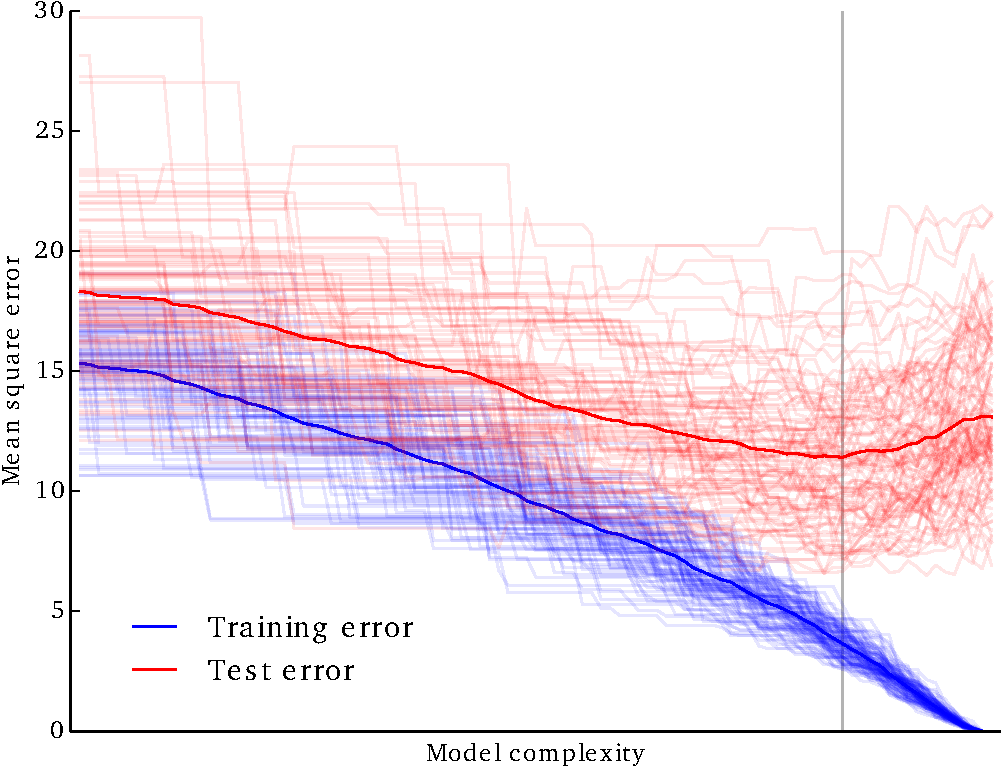
\includegraphics[width=.5\textwidth]{figures/chapter02/ch2_train_test_error.pdf}
  \caption{This plot is taken from \citet{louppe2014understanding}.
  The light blue curves show the training error while the
  light red curves show the estimated test error for 100
  pairs of training and test sets drawn at random
  from a known distribution. The thick blue curve is the average
  training error while the thick red curve is the average test error.
  It shows the necessary trade-off between the model's complexity and generalisation performance. As the model gets too complex, it starts overfitting the training data, decreasing test performance.}
  \label{fig:ch02:learning_curves}
\end{figure}
The attentive reader will notice that machine learning (ML) was only mentioned once until now, when discussing the Bayesian and frequentist interpretations of probability.
This may sound surprising as this thesis aims to build bridges between ML algorithms and the classical modelling approach. We did this on purpose as the distinction between classical modelling (as performed by domain experts, e.g. in science or engineering) and ML is often irrelevant. We have described probabilistic modelling in generic terms that are valid for both approaches. Whether the class of models is small, made of well-understood pieces, or a huge neural network does not matter when describing the key steps to building and using a model. Even a model designed with domain knowledge usually has degrees of freedom to adapt the model to contexts. At the same time, we must not forget that learning relies on assumptions even when using deep learning with large datasets.

% The Bayesian prospect allows drawing many connections between classical modelling and ML. For example, the Bayesian interpretation of the inductive bias of a machine learning algorithm can explain its generalisation property.
Classical modelling and machine learning aim to find the model that generalises well.
On the one hand, classical modelling generally considers simple classes of models which naturally aligns with Occam's razor. It often leads to faithful models when the studied process is well understood. On the other hand, machine learning tackles problems for which classical modelling would fail because the studied phenomenon is less well understood. This does not mean ML's job is to learn a complex model of the phenomenon, quite the opposite. As depicted in \Cref{fig:ch02:learning_curves}, an ML model achieves its best predictive performance by balancing the model's complexity and goodness of fit. This behaviour is arguably observed with all ML algorithms, although defining the model's complexity is not always straightforward. A standard method to control the complexity of an ML model is to split the data into training, validation and test sets. The validation set is used to find the hyperparameters of the learning algorithm that lead to a trained model that generalises well, that is, a model that has a good balance between faithfulness (good predictive accuracy for the task of interest) and complexity. We then use these hyperparameters to learn a new model with both train and validation sets and the test set to assess how well the model generalises.

Machine learning algorithms are sometimes described in deterministic terms. For example, a classical ML task is to predict a real value $y$ provided a set of features $\bm x$. At first glance, we might have trouble interpreting this in the probabilistic framework, limiting the scope of our previous discussion to a subset of ML algorithms. However, we can always map a deterministic model into the probabilistic framework. Indeed, deterministic learning objectives correspond to the MAP or the MLE of a probabilistic model that assumes the uncertainty a priori. For example, fitting a regression model $f_{\bm {\theta}}: \mathcal{X} \rightarrow \mathcal{Y}$ with mean squared error would lead to the same model as learning a probabilistic model via the MLE and considering a family of models that are Gaussian distributions with a fixed variance and a mean parameterised by $f_{\bm {\theta}}$. Similarly, mean absolute error corresponds to a Laplace distribution. The duality between the deterministic and the probabilistic interpretations goes further if we observe that regularisation strategies correspond to the prior in the MAP, e.g. ridge regression assumes a Normal prior on the coefficients of the linear model.

Another important aspect of modelling is to select the appropriate class of models. This choice varies with the end application which may require performing distinct types of queries on the model. In addition, the learning scenario may also differ and impacts the suitability of different models. As we will see soon, different models may lead to different inference algorithms. Some models represent the distribution of interest as a sampling procedure, while others provide access to the probability distribution. If our goal is to generate samples, we might prefer the former models, although we could also use Markov chain Monte Carlo to draw samples. The following sections shed light on popular classes of probabilistic models that exhibit different advantages and shortcomings.
%
% Things to mention:
% - Why we need train/valid/test (also for probabilistic); Provide the complexity plot.
% - Why using MSE or L1 error is equivalent to maximizing likelihood and adding a penalty to the parameters is equivalent to MAP.
% - How do we chose the learning algorithms/class of models? This a function of what we want to achieve with the model.

\section{Probabilistic graphical models}
As the saying goes, a picture is worth a thousand words. It is why we start our journey in the probabilistic-model lands by revisiting probabilistic graphical models (PGMs). Our trip will pass by Bayesian networks and make a slight detour by Markov networks, hoping to not leave the interested reader on the side of the road. As their name hints, PGMs rely on a graphical representation of the probability distributions. We will observe that directed and undirected graphs are appropriate to represent known (in)dependence relations. These representations lead to specialised inference and learning algorithms which will be discussed after.

The introduction of an undirected representation of the distribution of interacting particles in 1902 by Gibbs might be one of the first PGM. We can also attribute one of the first directed PGM to Sewall Wright, who introduced path analysis in genetics in the 1920s. The statistics community only started to acknowledge the graphical framework in the 1960s. And even later, in the late 80s, PGMs began to creep into the field of artificial intelligence (AI) with the seminal works of Judea Pearl and his colleagues that provided algorithms to take advantage of Bayesian networks, a class of directed PGMs. Since then, many communities have recognised the graphical representation as a powerful tool. It has achieved great success, such as in the modelling of gene regulatory networks~\citep{werhli2007reconstructing}, data compression~\citep{mceliece1998turbo}, and many others. Recently, causality, which under some aspects builds upon Bayesian networks, has arguably become one of the hottest topics in ML and might be part of the next successes in AI.

Many great resources on PGMs exist, and we do not pretend to compete with them. We aim to provide sufficient materials to get the reader interested in PGMs and understand standard algorithms' main advantages and limitations. This provides a common ground between the reader and the author to motivate the connections with deep probabilistic models and improvements to classical PGMs we have brought into the scope of this thesis. We invite the reader interested in additional details to check \citet{koller_probabilistic_2009}, the primary reference used to guide this introduction to PGMs.

\subsection{The curses of dimensionality}
% \textcolor{red}{add a figure that shows how the distance between two random points grows as the number of dimension grows.}
\paragraph{Learning is hard.} We consider a bunch of unfair coins $X = \left[X_1, \dots, X_d \right]^T$. Given a dataset of simultaneous throws $\mathcal{D} = \{\bm{x}_i\}_{i=1}^N$ , we want to learn a probabilistic model $P(X)$. A natural approach is to represent the joint probability as a $d$-dimensional array with an entry for each possible realisation. In this context, learning corresponds to filling the $2^d$ values in the table. We can reduce this number by factorising the distribution as
$$P(X) = P(X_1)\Pi_{i=2}^d P(X_i\mid X_1, \dots, X_{i-1}),$$ and by acknowledging that the (conditional) probabilities of a tail and a head sum up to $1$. Unfortunately, we do not gain much as the number of entries in the table still grows exponentially ($\sum_{i=1}^d 2^{i-1} = 2^{d-1} - 1$) and learning still quickly gets very difficult with the number of dimensions. This phenomenon is broadly referred to as a \textit{curse of dimensionality} and also hits continuous variables. However, this is just a recall to reality as we always need assumptions to create models. The good news is that we can fight the curse of dimensionality with modelling assumptions. For example, it is reasonable to assume the coins independent, the joint distribution is then factorized into $d$ terms: $ P(X) = \Pi_{i=1}^d P(X_i)$. For continuous variables, smoothness and constraints on the possible interactions between variables may allow us to achieve modelling results that challenge the curse of dimensionality. Soon, we will see strategies to express different modelling assumptions.
% - If we do not restrain the hypothesis space or bias the learning in some sense the curse of dimensionality kills us. -> Learning is hard.

\paragraph{Sampling is hard.} We want to sample realisations provided the joint distribution $P(X)$. To this end, we may use approximate sampling schemes (e.g., MCMC or importance sampling) that rely on a proposal distribution (e.g., a normal distribution) and an acceptance/rejection strategy. As the number of dimensions increases, the gap between the proposal distribution and the one of interest will naturally grow, and the acceptance rate will collapse. This means we must understand some modelling assumptions to develop an efficient sampling strategy. We will see later how rewarding is the joint development of the model class and the sampling strategy.

\paragraph{Interpreting is hard.} The complexity of a model naturally grows with the number of variables we consider. Clearly, humans are not able to apprehend correctly more than a few dimensions. If our goal is to understand how different modelling assumptions impact the model it may be important to use a specific framework for this. We will see that graphical models offer a nice balance between expressivity and interpretability.

\subsection{Directed graphical models - Bayesian networks}
Without appropriate assumptions on the modelled distribution, probabilistic modelling is hopeless in high dimensions for the reasons aforementioned. We now introduce Bayesian networks (BNs), which fight this intractability with independence assumptions. As we have seen, representing $d$ simultaneous coins tosses requires the specification of at least $2^{d-1} - 1$ numbers. This number drops to $d$ if we consider all the variables independent, which is reasonable as the realisation of one coin toss does not impact the outcome for another coin. BNs explicit these (conditional) independencies with a graphical representation and help parameterise distributions more compactly. The term Bayesian can be attributed to the Bayes' rule, which factorises the joint distribution into compact factors that encode the dependence between variables represented by the graph.

\subsubsection{Bayesian networks}
\begin{figure}[h]
    \centering
    \begin{subfigure}{.45\textwidth}
        \centering
        \begin{tikzpicture}[
          node distance=.7cm and 1.cm,
          var_x/.style={draw, circle, text width=.4cm, align=center}
        ]
            \node[var_x] (x1) {$X_1$};
            \node[var_x, right=of x1] (x2) {$X_2$};
            \node[var_x, below=of x1] (x3) {$X_3$};
            \node[var_x, right=of x3] (x4) {$X_4$};
            \path (x1) edge[-latex] (x2);
            \path (x1) edge[-latex] (x3);
            \path (x1) edge[-latex] (x4);
            \path (x2) edge[-latex] (x3);
            \path (x2) edge[-latex] (x4);
            \path (x3) edge[-latex] (x4);
            %\node (b) at (1,-3) {(\textbf{b})};
        \end{tikzpicture}
        \caption{}\label{fig:BN-fig-a}
    \end{subfigure}~\hspace{-4.8em}
    \begin{subfigure}{.45\textwidth}
    \centering
        \begin{tikzpicture}[
          node distance=.7cm and 1.cm,
          var_x/.style={draw, circle, text width=.4cm, align=center}
        ]
            \node[var_x] (x1) {$X_1$};
            \node[var_x, right=of x1] (x2) {$X_2$};
            \node[var_x, below=of x1] (x3) {$X_3$};
            \node[var_x, right=of x3] (x4) {$X_4$};
            %\node (a) at (1,-3) {(\textbf{a})};
            \path (x1) edge[-latex] (x3);
            \path (x1) edge[-latex] (x4);
            \path (x2) edge[-latex] (x3);
            \path (x2) edge[-latex] (x4);
        \end{tikzpicture}
        \caption{}\label{fig:BN-fig-b}
    \end{subfigure}
    \caption{Two Bayesian networks of a $4$D variable. (\textbf{a}) No independence. (\textbf{b}) A couple of independencies, hence a reduced number of edges and of parameters.} \label{fig:BN-fig}
\end{figure}

A Bayesian network is a directed acyclic graph (DAG) that represents independence assumptions between the components of a random vector. Formally, let $X = \left[X_1, \hdots, X_d\right]^T$ be a random vector taking values $\bm{x} \in \mathcal{X}_1 \times \dots \times \mathcal{X}_d$ distributed under $P(X)$. A BN for $X$ is a directed acyclic graph with one vertex for each random variable $X_i$ of $X$. In this network, the absence of edges models conditional independence between groups of components through the concept of d-separation~\citep{geiger_d-separation_1990}. A BN is a valid representation of a random vector $X$ iff its probability distribution (continuous or discrete) factorizes as
\begin{align}
    P(X) = \prod^d_{i=1}P(X_i\mid \mathcal{P}_i),\label{eq:BN-fact}
\end{align}
where  $\mathcal{P}_i = \{X_j: A_{j, i} = 1 \}$ denotes the set of parents of the vertex $i$ and $A \in \{0, 1\}^{d\times d}$ is the adjacency matrix of the BN. A BN, together with the related conditional probability distributions, is a PGM. For simplicity, we will use the term BN to refer to this couple and explicitly mention the terms topology or structure when talking about the BN's structure.

\Cref{fig:BN-fig-a} is a valid BN for any distribution over $X$ as it does not state any independence and leads to the chain rule factorization. However, in practice, we seek a sparse and valid BN which models most of the independence between the components of $X$, leading to an efficient factorisation of the modelled probability distribution. It is worth noting that making hypotheses on the graph structure is equivalent to assuming certain conditional independencies between some of the vector's components.

Understanding the independence assumptions underlying a DAG is key to appreciating BNs. For this purpose, d-separation describes rules to check whether a certain conditional independence holds in all distributions that factorise over a DAG. This algorithm is described in \Cref{alg:d-separation} and allows checking whether the topology is well suited to model a phenomenon of interest. In addition, it also enables characterising all (conditional) independencies that follow from a set of distinct independence assumptions. D-separation is \textit{sound}, it only detects existing independencies. However, it is not \textit{complete} as it misses independence assumptions hidden in the parameterisation of conditional distributions. For example, the BN in \Cref{fig:BN-fig-a} can model any joint distribution for $X$; applying d-separation to this graph would reject all independence, even though the distribution modelled could satisfy some independence relations.

\begin{algorithm}
\caption{D-separation.}\label{alg:d-separation}
  \begin{algorithmic}
    \Function{IsIndependent}{$X$, $Y$, $Z$, $G$}
      \State \Comment{\small $X, Y \text{ and } Z$ are three sets of nodes from $G$.}
      \State \Comment{\small Return True iff $X \indep Y \mid Z$ is modelled by the Bayesian network with topology $G$.}
      \State $A \gets \Call{AllAncestorsOf}{Z, G}$
      \For{$P_i \neq P_j \in A$} \Comment{\small Getting rid of immoralities.}
        \If{$\Call{HasACommonChild}{P_i, P_j, G}$}
          \State $G \gets \Call{AddUndirectedEdge}{P_i, P_j, G}$ \Comment{\small Marry parents.}
        \EndIf
      \EndFor
      \For{$N \in Z$}
        \State $G \gets \Call{RemoveNode}{N, G}$
      \EndFor
      \State \Return{\Call{IsNotReachable}{$X$, $Y$, $G$}}
    \EndFunction
   \end{algorithmic}
\end{algorithm}

\subsubsection{Parameterisation}
BNs reduce the description of a joint distribution into 1) a topology and 2) a batch of conditional distributions. As mentioned earlier, learning aims at selecting (or weighting) within a class of models. A natural way to define a model class is to use parameters to describe the free parts of the model. For BNs, domain knowledge often prescribes the topology, while learning the conditional distributions from data is more common. Moreover, it is simpler to parameterise and learn (conditional) distribution than graph structures that are discrete objects.

For discrete variables, we use categorical distributions, and each conditioning factor corresponds to distinct parameter values in the worst case. Continuous variables offer many alternative parameterisations, e.g. one distribution from the exponential family together with linear functions that compute the natural parameters given the conditioning factors. Gaussians with linear interactions are arguably one of the most popular parameterisations. These models, dubbed Gaussian Bayesian networks, were historically the only ones with an efficient training algorithm as they correspond to multivariate Gaussian distributions \citep{wermuth1980linear} for which closed-form MLE exists. In \Cref{ch:06}, we introduce normalizing flows as a more expressive parameterisation.
\subsubsection{Inference}
Almost any task we may want to perform on a model can be cast as inference. Here we focus on the generic the conditional probability query $P(Y\mid E=\bm{e})$, where $Y$ denotes a subset of the model's variable and $\bm{e}$ is the value of another subset $E$ of the variables, the remaining variables $M = \{X_i: X_i \notin Y \cup E \}$ are marginalised out. For example, we might be interested in evaluating $P(X_1\mid X_3=x_3, X_4=x_4)$ in \Cref{fig:BN-fig}.

\paragraph{Exact inference.}
As mentioned earlier, inference gets more complicated when the number of variables increases. However, BN adds structure to this problem by making some of the independencies explicit. While inference in BN stays NP-hard in the worst case, there exist algorithms able to exploit the structure for most inference tasks efficiently. For example, Pearl's message-passing algorithm is an efficient exact inference algorithm for polytrees, a subclass of BNs that have acyclic skeleton. Variable elimination (VE) is another popular algorithm that works on all discrete BNs and reduces the complexity of inference to the width (maximum distance between two nodes) of the graph. \citet{sanner2012symbolic} adapts VE to continuous variables with a symbolic version of VE. However, VE uses marginalisation and distribution products, which are not straightforward operations in the continuous setting.

\paragraph{Inference as sampling.}
The case of continuous variables motivates us to formulate inference differently. We look for formulations that do not explicitly mention marginalisation or the product of densities. A solution is to replace exact inference with conditional sampling from $P(Y\mid E=\bm{e})$. In BNs, \textit{Ancestral sampling} (AS) draws samples from the joint distribution by traversing the graph from parents to children and attributing a value to each node by sampling conditionally on the parents' values. AS can thus perform inference if the conditioning variables are ancestors of all variables in $Y$.

Ancestral sampling draws samples from each factor $P(X_i\mid \mathcal{P}_i)$ which is usually straightforward. For example, provided the corresponding cumulative distribution (CDF) function $F(\cdot;\mathcal{P}_i): \mathcal{X}_i \rightarrow \left[0, 1 \right]$ and a uniform random variable $U$ in $\left[0, 1\right]$, $x_i=F^{-1}(u;\mathcal{P}_i)$ follows $P(X_i\mid \mathcal{P}_i)$. This method is known as \textit{inversion sampling}.

\textit{Rejection sampling} (RS) is an alternative to inversion sampling, for example, when we cannot evaluate the inverse CDF directly. The idea is to sample $z \in \mathcal{X}_i$ from a proposal distribution $P_z$ and $u$ from a uniform between $0$ and $1$, then accept the sample if $u< \frac{p_{x_i}(z)}{K P_z(z)} $ where $K$ is chosen such that $ K P_z(x_i) \geq P_{x_i}(x_i) \quad \forall x_i \in \mathcal{X}_i$. RS works for multidimensional variables even when the joint distribution is only known up to a normalising factor. In that sense, it has more broadly applicable than IS. However, it becomes inefficient as the number of dimensions grows. Another limitation appears if we want to condition on a subset of the sampled variables, in which case the rejection rate blows up with the number of possible values for the conditioning variables (e.g., an infinite number in the continuous setting).

 Another possibility called likelihood weighting (LW) consists in freezing the conditioning factors $E$ to their value $\bm{e}$ and to sample values $(\bm{y}_1, \bm{m}_1), \dots, (\bm{y}_k, \bm{m}_k)$ via AS. These samples does not follow $P(Y, M\mid E=\bm{e})$ however we may approximate the expected value of a function $g$ with respect to $P(Y\mid E=\bm{e})$ by keeping track of the corresponding weights $P(Y, M, E=\bm{e})$ given by \Cref{eq:BN-fact}. The approximation of the expected value takes the following form
$$ \mathbb{E}_{P(Y\mid E=\bm{e})}\left[g(y)\right] \approx \frac{\sum_{i=1}^k g(\bm{y}_i) P(Y=\bm{y}_i, M=\bm{m}_i, E=\bm{e})}{\sum_{i=1}^k P(Y=\bm{y}_i, M=\bm{m}_i, E=\bm{e}) }.$$

For discrete variables, LW provides an approximate alternative to VE as
 $$P(Y=\bm{y}\mid E=\bm{e}) \approx \frac{\sum_{i=1}^k P(Y=\bm{1}\{y_i = y\}, M=\bm{m}_i, E=\bm{e})}{\sum_{i=1}^k P(Y=y_i, M=\bm{m}_i, E=\bm{e})}. $$
 This method is known as \textit{likelihood weighting} and is a special case of \textit{importance sampling} when the proposal distribution is ancestral sampling. Likelihood weighting is more efficient if the conditioning factors are close to the root of the BN.

Importance sampling does not provide iid samples from the posterior distribution, but Markov Chain Monte Carlo (MCMC) (with independent resampling) does. MCMC is a family of sampling algorithms that only require an unnormalised distribution. These algorithms run a Markov chain whose stationary distribution follows the given distribution. Each MCMC algorithm defines its own transition probability $P(Y^k\mid Y^{k-1})$. Many instances exist, such as Metropolis-Hastings MCMC, Hamiltonian MCMC, slice sampling, etc. Gibbs sampling is an instance that exploits the BN structure in the transition probability. Let us suppose that $M$ is empty, then at each transition step, Gibbs sampling only updates one component $Y_i$ of the vector $Y^k$. In particular, it samples $Y_i$ from the posterior $P(Y_i\mid Y_{-i}^{k-1})$ where $Y_{-i}^{k-1}$ contains the values of the evidence $E$ and the previous state $Y^{k-1}$ except the $i^{\text{th}}$ component.

% \textcolor{red}{Mention that we do not pretend to be complete as there exist many many algorithms and we only focus on generic algorihm that showcase some of the classical issuing when sampling from these models. I have to help the reader to understand better why he it is important that he reads this sections. For the one about sampling it shows that inference is really hard but adding strucure helps producing specialized algorithms. For the inference as optimization it must mainly motivates to create parametric models that are efficiently trainable. Also mention that although we try to keep the discussion generic, our interest is really for continuous variables in this thesis. Find a place to mention the Expectation–maximization algorithm.}

\paragraph{Inference as optimization.}
We finally introduce variational inference (VI) as a third alternative for inference. VI formulates inference as an optimisation problem in which we look for a distribution $Q(Y)$ that is as close as possible to the posterior of interest $P(Y\mid E=\bm{e})$. For this purpose, we consider a parametric family of distributions $Q_{\bm{\theta}}(Y)$, such as a BN with a prescribed structure but parametric distributions. Our goal is to optimise for the best set of parameters $\bm{\theta}^\star$:
\begin{align}
  \bm{\theta}^\star = \argmin_{\bm{\theta}} \mathbb{D}\left[Q_{\bm{\theta}}(Y)\Vert P(Y\mid E=\bm{e}) \right], \label{eq:obj_VI}
\end{align}
where $\mathbb{D}$ is an appropriate divergence between distributions. For the rest of this discussion, let us fix $\mathbb{D}$ to the Kullback-Leibler ($\mathbb{KL}$) divergence which is an appropriate choice as it is only minimized when $Q = P$. As of now, we also restrain our discussion to the case of continuous variables. Formally, the $\mathbb{KL}$ compares two distributions $P(X)$ and $Q(X)$ as $$\mathbb{KL}\left[P\Vert Q\right] \triangleq \int_{\bm{x} \in \mathcal{X}} P(\bm{x}) \log \frac{P(\bm{x})}{Q(\bm{x})} \text{d}\bm{x}$$. The integral can be replaced by a sum for discrete random variables. The $\mathbb{KL}$ is not a propper distance as it is not symmetric.

Solving $\Cref{eq:obj_VI}$ is possible if we have a parametric family of distributions for which density evaluation and sampling are differentiable functions of the parameters. This family could be another BN or a Normalizing flow, a deep probabilistic model we describe in the next section. Let us denote by $Q_{\bm{\theta}}$ the probability density function and the procedure to generate samples as $$ y := f_{\bm{\theta}}(z) \quad\text{where}\quad z\sim \mathcal{N}(0, I),$$
where $\mathcal{N}(0, I)$ denotes a normal distribution.
In this ideal case, the optimization problem becomes:
\begin{align}
  \bm{\theta}^\star &= \argmin_{\bm{\theta}} \mathbb{KL}\left[Q_{\bm{\theta}}(Y)\Vert P(Y\mid E=\bm{e}) \right]\\ \label{eq:VI_optim}
  &= \argmin_{\bm{\theta}} \mathbb{KL}\left[Q_{\bm{\theta}}(Y)\Vert P(Y, E=\bm{e}) \right] + \mathbb{E}_{\bm y}\left[\log P(E=\bm{e})\right]\\
  &= \argmin_{\bm{\theta}} \mathbb{E}_{z}\left[ \log \frac{Q_{\bm{\theta}}(f_{\bm{\theta}}(z))}{P(f_{\bm{\theta}}(z), E=\bm{e})} \right].
\end{align}
We can optimise this equation with stochastic gradient descent (SGD) by approximating the objective function with Monte Carlo samples at each gradient step.

Evaluating $P(f_{\bm{\theta}}(z), E=\bm{e})$ in the last equation is not always possible (e.g.; if the variables in $M$ are not leaves). In this context, we may create an approximation $Q_{\bm{\theta}^\star}(Y, M\mid E=\bm{e})$ of $P(Y, M\mid E=\bm{e})$ instead. We can then generate samples from the joint and thus from the marginal $P(Y\mid E=\bm{e})$. If we need to evaluate the approximate
$$Q_{\bm{\theta}^\star}(Y\mid E=\bm{e}) := \int_{\bm{m} \in \mathcal{M}} Q_{\bm{\theta}^\star}(Y, M=\bm{m}\mid E=\bm{e}) \text{d}\bm{m}$$, we can find a surrogate model $\tilde Q_\psi$ by solving the following optimization problem:
\begin{align}
  \psi^\star &= \argmin_\psi \mathbb{KL}\left[Q_{\bm{\theta}^\star}(Y, M\mid E=\bm{e})\Vert \tilde Q_\psi(Y) \right]. \label{eq:approx_posterior}
\end{align}
We can also optimize this equation with SGD and Monte Carlo samples as it only requires to sample from and evaluate $Q_{\bm{\theta}^\star}(Y, M\mid E=\bm{e})$, and to evaluate $Q_\psi(Y)$. We can convince ourselves that the solution to \Cref{eq:approx_posterior} corresponds to $Q_{\bm{\theta}^\star}(Y\mid E=\bm{e})$,
\begin{align}
  &\argmin_Q \mathbb{KL}\left[P(Y, M)\Vert Q(Y) \right]\\
  &=\argmin_Q \mathbb{E}_{P(Y) P(M\mid Y)}\left[\log P(Y) + \log P(M\mid Y) - \log Q(Y)\right]\\
  &=\argmin_Q \mathbb{E}_{P(Y) P(M\mid Y)}\left[\log P(Y) - \log Q(Y)\right]\\
  &= \argmin_Q \mathbb{E}_{P(Y)}\left[\log P(Y) - \log Q(Y)\right]\\
  &= \argmin_Q \mathbb{KL}\left[P\Vert Q \right].
\end{align}

We observe that VI can only achieve good results if the family of distributions contain instances close to the true posterior. In addition, solving the optimisation can be complicated even if provided with a parametric universal density approximator. However, VI is often preferable to sampling strategies for multiple reasons. It eventually becomes faster than sampling as \Cref{eq:obj_VI} returns a model from which we can generate as many samples as wanted. This approach also automatically provides a surrogate of the posterior density. Finally, we can apply this approach to learning a parametric posterior distribution that approximates $P(Y\mid E=\bm{e})$ for any value of $e$.

Another interesting application of VI is for estimating a bound on the log-marginal $\log P(E)$ of the larger model $P(Y, E)$. We can directly derive from \Cref{eq:VI_optim}:
\begin{align}
  \mathbb{KL}\left[Q_{\bm{\theta}}(Y)\Vert P(Y\mid E=\bm{e})\right] &\geq 0\\
  \mathbb{KL}\left[Q_{\bm{\theta}}(Y)\Vert P(Y, E=\bm{e}) \right] + \mathbb{E}_{y}\left[\log P(E=\bm{e})\right] &\geq 0\\
  \mathbb{E}_{\bm y \sim Q_{\bm{\theta}}(Y=\bm{y})}\left[ \log \frac{P(E=\bm{e}\mid Y=\bm{y}) P(Y=\bm{y})}{Q_{\bm{\theta}}(Y=\bm{y})} \right] &\leq \log P(E=\bm{e})\\
  \underbrace{\mathbb{E}_{\bm y \sim Q_{\bm{\theta}}(Y=\bm{y})}\left[ \log P(E=\bm{e}\mid Y=\bm{y})\right] - \mathbb{KL}\left[Q_{\bm{\theta}}(Y)\Vert P(Y)\right]}_{\operatorname{ELBO}} &\geq \log P(E=\bm{e}) \label{eq:elbo}
\end{align}
This estimated lower bound on the evidence ($\operatorname{ELBO}$) is useful to approximate the log-likelihood of a parametric model $P_{\bm \psi}(E)$ defined as the marginal of a larger model $P_{\bm \psi}(Y, E)$.
We will see how VI allows learning deep probabilistic models that formulates the generative process as a stochastic map from latent variables to observations.
% \textcolor{red}{Discuss the case of exact inference in continuous is maybe hopeless.}
\subsubsection{Learning}
With VI, we have seen for the second time that inference and learning are two faces of the same coin. We now describe learning strategies to fit the parameters of a BN given data.
A BN combines a graph $G \in \mathcal{G}$, where $\mathcal{G}$ denotes the set of DAGs, and $\mathcal{F} = \{P_{\bm{\theta}_i}(X_i\mid \mathcal{P}_i)\}_{i=1}^d$ is the corresponding set of parametric conditional distributions that together model a joint distribution. Ideally, we would like to adapt both $G$ and $f_{\bm{\theta}} \in \mathcal{F}$ to the learning dataset $\mathcal{D}=\{X^i\}_{i=1}^N$.

Assuming iid data, we can express the learning task as a generic optimisation problem:
\begin{align}
  B^\star  = \argmax_{B\in\mathcal{B}} \sum_{i=1}^N \log P_B(X^i) - R(B), \label{eq:learn_BN}
\end{align}
where $\mathcal{B} = \mathcal{G} \times \mathcal{F}$ denotes the set of possible BNs and $R(\cdot): \mathcal{G} \times \mathcal{F} \rightarrow \mathbb{R}$ is a regularisation term which can be interpreted as the prior over plausible BNs and is constant if we do MLE. We insist on the importance of $R(B)$ for obtaining a good model. Although BNs with complete DAGs are strictly more expressive than sparse structures, we prefer the latter as they explicit independence assumptions and lead to simpler conditional distributions.

The formulation in \ref{eq:learn_BN} does not say much about concrete strategies to fit the parameters of a BN. In practice, we often separate structure learning from distribution fitting. Structure learning is a combinatorial problem, whereas fitting the parameters of conditional distributions is a continuous optimisation problem; solving both issues jointly is an open problem. In \Cref{ch:06}, we will see one strategy to formulate the combinatorial problem into a continuous one; these are advanced concepts beyond this background's scope. Now, we focus on the two sub-problems independently.

\paragraph{Distribution learning.}
We suppose a prescribed topology and only focus on learning the best factors in \Cref{eq:BN-fact}. For this purpose we can parameterize the factors with a vector $\bm \theta := \left[\bm{\theta}_1, \cdots, \bm{\theta}_d\right]$ and update \Cref{eq:learn_BN} into
\begin{align}
  {\bm \theta}^\star  = \argmax_{\bm \theta} \sum_{i=1}^N \log \prod^d_{j=1}P_{\bm \theta}(X_j^i\mid \mathcal{P}_j) - \log \pi(\bm \theta).
 \label{eq:learn_factors}
\end{align}
In practice, we approach ${\bm \theta}^\star$ via stochastic gradient ascent on the objective of \Cref{eq:learn_factors}.
The choice of the parameterisation and the prior $\pi$ are crucial to finding a good model when $N$ is finite.
% Although parametric universal density approximators exist, such as normalizing flows, learning the parameters of these functions can be challenging when the dataset is small or the phenomenon modelled is complex. The optimisation problem described by \Cref{eq:learn_factors} is usually solved via stochastic gradient descent.

\paragraph{Structure learning.}
It is sometimes difficult to define a relevant structure a priori, and it may be interesting to learn it from data instead. Structure learning aims to find a sparse topology that does not imply (conditional) independence in contradiction with the data. We can formulate this search as an optimisation problem under constraints in the space of DAGs $\mathcal{G}$:
\begin{align}
 G^\star = \argmin_{G \in \mathcal{G}} \sum_{i=1}^d\sum_{j=1}^d A_{i,j}(G) \quad \text{such that} \quad I(G) \subseteq I(\mathcal{D}), \label{eq:learn_structure}
\end{align}
where $A(G)$ is the adjacency matrix of the graph $G$, $I(G)$ is the set of (conditional) independence encoded by $G$, and $I(\mathcal{D})$ is the set of independence observed in the data. The constraints ensure that only independencies observed in the data are encoded in the structure, and the objective penalizes the number of edges.

Fixing the topological ordering in advance reduces drastically the size of the search space and allows greedy algorithms. In this case, the solution's quality depends on the chosen order. In addition to being intractable, the formulation in \Cref{eq:learn_structure} does not take advantage the prior knowledge. A partial solution is to reduce the search space $\mathcal{G}$ to the structures we consider plausible. Expressing more subtle priors over graphs and handling them efficiently in structure learning is still an open research question.

The evaluation of $I(\mathcal{D})$ is essential for structure learning. In theory, testing for independence in the data is difficult as it requires accessing the (conditional) distribution between the two variables tested, which is what we are trying to learn. In practice, we create statistical independence tests by making assumptions on the class of interactions and marginal distributions (e.g. linear Gaussian, discretisation of variables, etc.). These tests are reasonably accurate for unconditional independence but not for conditional independence. Interestingly, while pure independence between continuous variables is hard to prove in practice, it is often beneficial to consider weakly dependent variables as if they were independent. This usually simplifies the model and improves its generalisation to unseen data.

In parallel to this, there exist specialized algorithms for learning BNs' structures. Some implement greedy solutions which provide a useful approximation of the true solution~\citep{tsamardinos2006max}. Others focus on sub-class of BNs for which efficient solutions exist~\citep{cooper1992Bayesian, chow1968approximating}. In general, topology learning is a tough problem but has recently regained great attention from the machine learning community in the context of causal discovery~\citep{khemakhem_causal_2020, balgi2022counterfactual, vowels2021d, brouillard2020differentiable}.


\subsubsection{Duality between directed graphs and distributions}
If a distribution $P$ factorises over a Bayesian network with graph $G$, we can check whether some conditional independence holds with d-separation. In this case, we say that the Bayesian network is an \textit{I-map} of the independence in $P$ - any independence expressed by the BN is present in $P$. However, we have also observed that any distribution factorises over the complete graph. Complete Bayesian networks are unsatisfactory as they do not reflect any independence assumptions necessary for manipulating the distribution efficiently.

Our goal is thus to find a sparse graph that only represent independence present in the distribution we aim to model. In particular, we say that a graph $G$ is a \textit{minimal I-map} for a set of independencies if it is an I-map and if the removal of even a single edge breaks the I-map property. We are generally only interested in BNs that are an I-map of the modelled distribution. However, \textit{minimal I-map} are not perfect because they can miss some independencies in $P$. A graph $G$ is a \textit{P-map} for a set of independencies $\mathcal{I}$ if the independence modelled by the graphs $\mathcal{I}_G$ are equal to $\mathcal{I}$ - that is, any independence modelled by $G$ is in $\mathcal{I}$, and all independencies in $\mathcal{I}$ are modelled by  $G$.

Clearly, any P-map is a minimal I-map, and the best BNs are the one that are P-maps of the distribution of interest. Unfortunately, Bayesian networks are not universal P-maps. Some sets of independencies $\mathcal{I}$ are impossible to express faithfully with directed graphs. In such a case, either the graph misses some independence or expresses false independence. We will see that undirected graphs can represent faithfully such independencies but have other limitations and are not universal P-maps either.
\subsubsection{Causality}
It is natural to interpret the arrows in a BN as causal relationships between variables. This interpretation is dangerous as it is not necessarily correct. For example, two complete BNs with opposed arrows may express the same distribution but opposite causal relationships. However, causal graphs can be interpreted as BNs. In these graphs, a directed edge from $X$ to $Y$ represents the causation of $Y$ by $X$. The BN corresponding to a causal graph is an I-map of the distributions between the variables present in the causal graph.

We can recycle algorithms and interpretation from BNs to causal graphs but not vice-versa. We can also try to understand some algorithms by assuming the BN is a valid causal graph. For example, causality implies that we shall first sample parents to generate the children and provides a natural interpretation of the ancestral sampling algorithm. As we will see in the next section, some (in)dependence assumptions about the distributions are fundamentally non-causal, which hints at why BNs are not universal P-maps.

Causality has become a significant sub-field of artificial intelligence and strongly impacts machine learning. Do-calculus \citep{pearl1994probabilistic} is a tool that allows inference with causal rather than probabilistic facts. Such reasoning patterns are necessary to answer counterfactual questions scientifically. In addition, causal assumptions prove the generalisation and robustness of some machine learning algorithms. The recent interest in causal modelling provides additional motivations for using directed graphs, hence BNs, to model distributions. As said, this also inevitably contradicts some (in)dependence assumptions we may want to formulate and motivate the following discussion about undirected representations.
\subsection{Undirected graphical models - Markov networks}
We have shown with Bayesian networks that graph structures can represent important properties of probability distributions and lead to many specialised algorithms for learning and inference. The duality between Bayesian and causal networks provides a simple procedure to constrain the structure of the networks when we have a causal understanding of the studied process. However, the duality also implies that BNs are not universal P-maps, as shown in the following example. Let $X_1, X_2, X_3, X_4$ be four random variables related by the following independence statements: $\{ X_1 \indep X_3 \mid (X_2, X_4), X_2 \indep X_4 \mid (X_1, X_3)\}$. A Bayesian network cannot faithfully represent such independence statements. Indeed the assumptions impose that $X_2$ and $X_4$ d-separate $X_1$ and $X_3$ and vice versa. This imposes that the structure of the BN resembles \Cref{fig:MN-fig-b}. However, it is impossible to add directions to the edges without adding a cycle or a V-structure that would contradict at least one of the independence hypotheses.

This example is even more straightforward if we take a concrete example where such assumptions would be reasonable and observe that it contradicts the causal interpretation of BNs. Let us consider that the four random variables correspond to the opinion of four wine amateurs about a C{\^o}tes de Provence ros{\'e}. Each amateur tastes the wine twice, on two different days, with two distinct amateurs. As they discuss together, the opinion of each amateur is influenced by the view of the others and vice versa. Because we expect each pair to reach some consensus, all opinions should influence each other, sometimes indirectly.  Each amateur will have a final opinion about the wine eventually. This contradicts a causal interpretation in which one of the variables, the root, should not be influenced by another.

It sounds more natural to express similar configurations with an undirected graph. Undirected graphical models can indeed represent such conditional independence faithfully. However undirected graphs are not universal P-maps either as they cannot represent independence assumptions rooted in causal interpretation. For example, it is impossible to express that two independent variables can become dependent when conditioned on a third variable (V-structure in BNs) which naturally arises when the two independent variables cause the third. We briefly introduce these models, united under the term Markov networks. Our goal is only to provide some intuition about this class of models, as these graphical models are not directly related to any of the contributions in this thesis.
\paragraph{Markov networks.}
\begin{figure}
    \centering
    \begin{subfigure}{.45\textwidth}
        \centering
        \begin{tikzpicture}[
          node distance=.7cm and 1.cm,
          var_x/.style={draw, circle, text width=.4cm, align=center}
        ]
            \node[var_x] (x1) {$X_1$};
            \node[var_x, right=of x1] (x2) {$X_2$};
            \node[var_x, below=of x1] (x3) {$X_3$};
            \node[var_x, right=of x3] (x4) {$X_4$};
            \path (x1) edge[-] (x2);
            \path (x1) edge[-] (x3);
            \path (x1) edge[-] (x4);
            \path (x2) edge[-] (x3);
            \path (x2) edge[-] (x4);
            \path (x3) edge[-] (x4);
            %\node (b) at (1,-3) {(\textbf{b})};
        \end{tikzpicture}
        \caption{}\label{fig:MN-fig-a}
    \end{subfigure}~\hspace{-4.8em}
    \begin{subfigure}{.45\textwidth}
    \centering
        \begin{tikzpicture}[
          node distance=.7cm and 1.cm,
          var_x/.style={draw, circle, text width=.4cm, align=center}
        ]
            \node[var_x] (x1) {$X_1$};
            \node[var_x, right=of x1] (x2) {$X_2$};
            \node[var_x, below=of x2] (x3) {$X_3$};
            \node[var_x, left=of x3] (x4) {$X_4$};
            %\node (a) at (1,-3) {(\textbf{a})};
            \path (x1) edge[-] (x2);
            \path (x2) edge[-] (x3);
            \path (x3) edge[-] (x4);
            \path (x4) edge[-] (x1);
        \end{tikzpicture}
        \caption{}\label{fig:MN-fig-b}
    \end{subfigure}
    \caption{Two Markov networks of a $4$D variable. (\textbf{a}) No independence. (\textbf{b}) Cycle dependencies. A Bayesian network cannot represent all implied independencies but a Markov network can.} \label{fig:MN-fig}
\end{figure}
A Markov network (MN), also called Markov Random Field, is an undirected graph that describes \textit{Markov properties} between random variables. Formally, let $X = \left[X_1, \hdots, X_d\right]^T$ be a vector collecting the random variables, the global Markov property states that any two subsets of variables are conditionally independent given a separating subset $X_A \indep X_B \mid X_S$, where the subset of variables $X_S$ separates the subsets $X_A$ and $X_B$ - $X_S$ blocks all path from $X_A$ to $X_B$ in the graph. For example, the Markov network in \Cref{fig:MN-fig-a} does not impose any independence whereas the one in \Cref{fig:MN-fig-b} implies the following independence: $\{ X_1 \indep X_3 \mid (X_2, X_4), X_2 \indep X_4 \mid (X_1, X_3)\}$.

\begin{table}[h]

  \begin{subtable}[t]{.45\linewidth}
      \centering
  \begin{tabular}{c|cc|}
    \diagbox{$X_1$}{$X_2$}
  % \\diagbox[height=1\line]{\rlap{\enspace\raisebox{2ex}{$X_1$}}}{\raisebox{-3.5ex}{$X_2$}}
% \backslashbox{\tabular{@{}l@{}}$X_1$\endtabular}{$X_2$}
  & $0$& $1$ \\\hline
$0$ & $10$ & $30$ \\
$1$ & $50$ & $10$    \\\hline
\end{tabular}
  \caption{}
  \label{tab:MN_simple_factor}
\end{subtable}%
\hfill
\begin{subtable}[t]{.45\linewidth}
  \centering
\begin{tabular}{c|cc|}
  \diagbox{$X_1$}{$X_2$}
% \\diagbox[height=1\line]{\rlap{\enspace\raisebox{2ex}{$X_1$}}}{\raisebox{-3.5ex}{$X_2$}}
% \backslashbox{\tabular{@{}l@{}}$X_1$\endtabular}{$X_2$}
& $0$& $1$ \\\hline
$0$ & $0.1$ & $0.3$ \\
$1$ & $0.5$ & $0.1$    \\\hline
\end{tabular}
  \caption{}
  \label{tab:MN_simple_joint}
\end{subtable}%
\caption{The numerical values associated with a two nodes ($X_1$ and $X_2$) Markov network. (\textbf{a}) The unnormalised factor. (\textbf{b}) The factor normalised corresponds to the joint distribution.}
\end{table}
\paragraph{Parameterisation.}
Similar to BNs, the graphical structure of a Markov network describes independencies but does not explicit the exact distribution. For this Markov networks use factors, which are functions describing the interactions between connected variables. Unlike BNs, factors are unormalized and do not directly correspond to conditional distributions. Instead, they reflect the absolute strength of interaction between the variables. For example, let $X_1$ and $X_2$ be two binary random variables, \Cref{tab:MN_simple_factor} reports possible values for the factor $\phi(X_1, X_2): \{ 0, 1\} \times \{ 0, 1\} \rightarrow \mathbb{R}$. We can compute the corresponding joint distribution by summing and normalizing factors as
$$ P(X_1, X_2) = \frac{\phi(X_1, X_2)}{\sum_{(x_1, x_2) \in \{ 0, 1 \} \times \{ 0, 1\} } \phi(X_1=x_1, X_2=x_2)}. $$

We extend interactions between more than two variables with factors that parameterize the joint distribution of a random vector $X = \left[X_1, \hdots, X_d\right]^T$ as a set of factors $\bm{\phi} = \{ \phi_1(D_1), \dots, \phi_K(D_K) \}$ that defines an unormalised distribution as
$$ \tilde{P}_{\bm{\phi}(X)} = \phi_1(D_1) \times \dots \times \phi_K(D_K). $$
% A markov network factorizes such distribution if there is one factor for each group of variables that defines a complete subgraph. These subgraphs are called cliques.
The corresponding distribution is
$$P_{\bm{\phi}(X)} = \frac{1}{Z}\tilde{P}_{\bm{\phi}(X)},$$
where the normalising factor is $Z=\sum_{\bm{x} \in \mathcal{X}}\tilde{P}_{\bm{\phi}(X=\bm{x})}$ if the random vector is discrete or $Z=\int_{x \in \mathcal{X}}\tilde{P}_{\bm{\phi}(X=\bm{x})}\text{d}\bm{x}$ if it is continuous. Markov networks define a joint distribution with an unnormalised function that scores the plausibility of each possible realisation.

When the factors are stricly positive, the unnormalised distribution can be written as $$ \tilde{P}_{\bm{\phi}(X=\bm{x})} = e^{-E(\bm{x})}, $$ and E is dubbed the energy function. This family of distributions is called Gibbs distributions and factorises over a Markov network if each factor takes as input a clique, a complete subgraph of the network. Parameterising Markov networks can be cumbersome as the number of cliques grows with the complexity of the graph. In practice, we minimize the number of edges in the graph and only parameterise 1D and 2D factors.

\begin{figure}
    \centering
    \begin{tikzpicture}[
      node distance=2.cm and 1.5cm,
      var_x/.style={draw, circle, text width=.4cm, align=center},
      simple/.style={align=center}
    ]
        \node[var_x] (a) {$V_1$};
        \node[simple, right=of a] (b) {$\dots$};
        \node[var_x, right=of b] (c) {$V_m$};

        \node[var_x, below=of a] (w) {$H_1$};
        \node[simple, right=of w] (x) {$\dots$};
        \node[var_x, right=of x] (y) {$H_n$};

        \path (a) edge[-] (w);
        \path (a) edge[-] (x);
        \path (a) edge[-] (y);
        \path (b) edge[-] (w);
        \path (b) edge[-] (x);
        \path (b) edge[-] (y);
        \path (c) edge[-] (w);
        \path (c) edge[-] (x);
        \path (c) edge[-] (y);
        %\node (b) at (1,-3) {(\textbf{b})};
    \end{tikzpicture}
    \caption{A Restricted Boltzmann machines compose of $n$ hidden units $H_i$ and $m$ visible units $V_j$. The Markov network is a bipartite graph separating hidden and visible units into two groups fully connected to each other.}\label{fig:RBM}
\end{figure}

Provided the graph structure and factors, we can use sampling algorithms, such as MCMC, to generate realisations that follow the distribution modelled by the network. But without additional constraints on the structure manipulating these models is difficult.
Restricted Boltzmann machines (RBMs) are a popular class of Markov networks where binary variables are split into visible units, denoted $V \in \{0, 1\}^m$, and hidden units, $H \in \{0, 1\}^n$, with a bipartite graph as depicted in \Cref{fig:RBM}. This restriction allows efficient learning algorithms inspired by the Hebbian plasticity of the brain. The parameterisation of RBMs is a matrix of weights $W \in \mathbb{R}^{m\times n}$ that describes the interactions between visible and hidden units and two vectors of offset $\bm{b}_H$ and $\bm{b}_V$ respectively for hidden and visible units. The joint distribution between visible and hidden units is computed as
$$ P(V=\bm{v}, H=\bm{h}) = \frac{1}{Z} \phi(V=\bm{v}, H=\bm{h}), $$
where the factor is $ \phi(V, H)=e^{-E(V, H)} $ and the energy function takes the particular form
$$ E(V=\bm{v}, H=\bm{h}) = -\bm{b}_H^T \bm{h} - \bm{b}_V^T \bm{v} - \bm{v}^T W \bm{h}.  $$
We can train these networks on a dataset of visible variables with an algorithm that combines Gibbs sampling (on the hidden units) and gradient descent to update the weights. RBMs are among the first success of neural networks and have been used for unsupervised learning problems such as dimensionality reduction, collaborative filtering, and others.
% \paragraph{Markov versus Bayes.}
% Markov -> BN
% BN -> Markov
% \paragraph{Inference.}
%
% \paragraph{Learning.}
%
%
% \paragraph{Other graphical representations.}
% We naturally observe relationships between directed and undirected representations. While directed graphs can be interpreted in causal terms they do not require this intepretation. There is no fundamental obstacles to translate directed structures into undirected networks and vice versa.

\section{Deep probabilistic models}
RBMs are arguably one of the first generative models built upon neural networks. This section discusses other successful approaches for parameterising probabilistic models with neural networks. While graphical models describe probabilistic models with graphs and are appealing for understanding and prescribing modelling assumptions, they do not rigorously describe efficient parameterisations of the conditional probability distributions in the continuous setting. Deep probabilistic models encompass methods for parameterising these probability distributions with neural networks. Some of these models are particularly well suited for sample generation and are called \textit{deep generative models}. We will highlight the correspondence of some of these models within the probabilistic graphical models when possible.
\subsection{Why neural networks?}
We abstract neural networks as parametric functions that maps an input space $\mathcal{X}$ to an output space $\mathcal{Y}$ and are differentiable function $f_{\bm{\theta}}: \mathcal{X} \rightarrow \mathcal{Y}$ of its parameters $\bm{\theta}$. Although neural networks are universal function approximators, the parameterisation of a probability distribution is challenging and requires the right architectural choice. We often present neural networks as deterministic models; however, many strategies exist to parameterise probability distributions, as we will see in the next sections.

For example, Normalizing flows are neural networks that directly parameterise the probability distribution but require strong architectural constraints, as we will see later. This is particularly inconvenient when working with structured data (e.g. images, sound, graphs, etc.) because specialised architectures (e.g. convolutions) do not directly satisfy the architectural constraints. Another possibility is to use a neural network to parameterise a known distribution such as a Gaussian. For example, we can model $P(Y|X)$ as a multivariate Gaussian $\mathcal{N}(\bm{\mu}, \Sigma)$ where a free-form neural network computes the mean vector and covariance matrix as a parametric function of the input $X$. This strategy makes a strong assumption in the form of $P(Y\mid X)$, which may be inaccurate, e.g. if $X$ is a piece of text describing the image $Y$. An alternative is to see the neural networks as a generator of samples similar to the training set, mapping a noise vector to realisations. These deep generative models define the probability distribution implicitly and allow us to use complex architectures well suited to the modelling task but require specialised training algorithms, as we will see in the following sections.

Neural networks are better suited to parameterise distributions than other machine learning models. In particular, their differentiability and training procedure based on stochastic gradient descent allows us to optimise objectives corresponding to the MLE or MAP directly. In parallel, considerable effort has been made over the last year to create architectures with inductive biases adapted to different data types. The availability of large pre-trained models is another advantage of working with neural networks. For example, Dall-e 2~\citep{ramesh2022hierarchical} combines a large pre-trained language model with annotated images to train a text-to-image probabilistic model.

In the following we will mostly ignore the conditioning variable $X$ as challenges in modelling distributions with neural networks is usually orthogonal to handling conditioning variables. Instead we focus on the modelling of the joint distributions of a $d$-dimensional random vector $Y = \left[Y_1, \dots, Y_d  \right]$ that takes value in $\mathcal{Y} = \mathcal{Y}_1 \times \dots \times \mathcal{Y}_d$. For simplicity, we consider that $\mathcal{Y}_1 = \dots = \mathcal{Y}_d$ and the domains are either discrete classes (e.g. a pixel value in $\{0, \dots, 255\}^3$) or real numbers $\mathbb{R}$.
\subsection{Autoregressive models} \label{subsec:AM}
If Bayes' rule were a deep probabilistic model, it would be an autoregressive model. These models decompose the joint distribution as
\begin{align}
  P(Y) = P(Y_1) \Pi^d_{i=2} P(Y_i|Y_{<i}), \quad \text{where} \quad Y_{<i} \triangleq \left[ Y_1, \dots, Y_{i-1}\right].
\end{align}
When the domain is discrete, we can parameterise each $1$D factor with a classifier. If the domain is continuous, the common practice is to parameterise a $1$D Gaussian distribution with a neural network that predicts the mean and log-variance given the conditioning vector.
This naturally leads to the parameterization of $d$ functions with different input dimensionality which might be very inefficient if $d$ is large (e.g. $2^{16}$ for $256\times256$ images).

Sharing parameterisation between factors is an important aspect of autoregressive models. One strategy is to use recurrent neural networks where the hidden vector carries and updates the information of the successive conditioning variables\citep{van2016pixel}. However, this strategy is slow because it processes the input vector sequentially. Moreover, the inductive bias of recurrent neural networks is not ideal for signals with long-range or spatial dependencies such as audio or images. A better solution is to use causal convolutional neural networks (CNNs), which process the complete vector simultaneously and enforce the autoregressive structure in the outputs. Causal CNNs have achieved great success in modelling audio \citep{van_den_oord_wavenet_2016, van_den_oord_parallel_2018}. The PixelCNN autoregressive model generalises this architecture to 2D signals and has shown great modelling capabilities\citep{oord_conditional_2016}.

We can train autoregressive models efficiently by maximising their likelihood given data. Evaluating the likelihood only requires passing the data once in the network and computing the product of the $d$ conditional distribution evaluated at the input vectors. Unfortunately, sampling is a sequential process as each variable is sampled according to the preceding. This is particularly slow for images or long time series and is one of the main drawbacks of autoregressive models. The lack of independence assumptions and poor inductive bias are additional limitations of these models. This is especially true with images for which the enforced causality between successive pixels and sampling algorithm is ineffective. We rarely use autoregressive models alone but in combination with other models, such as variational auto-encoders.

% \textcolor{red}{Add an image that describes the sampling procedure of autoregressive nets.}
\subsection{Energy based models}
\begin{figure*}
  \centering
  \begin{subfigure}{.48\textwidth}
    \centering
    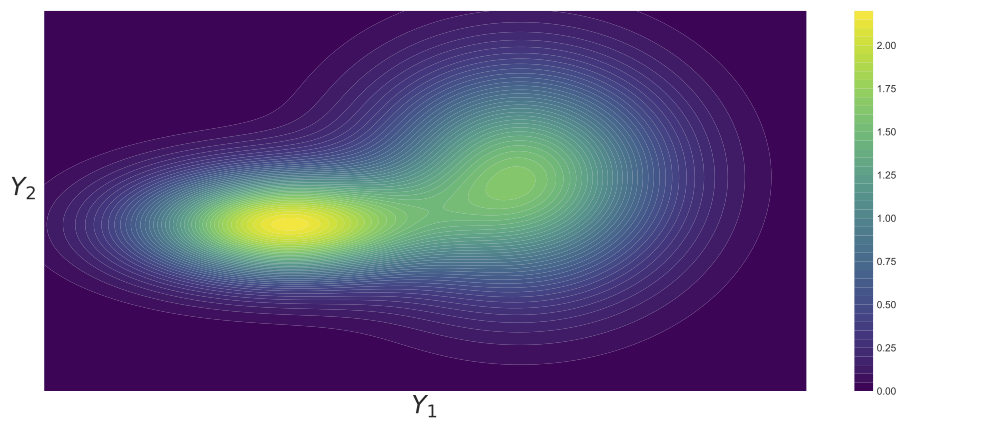
\includegraphics[width=.95\textwidth]{figures/chapter02/energy-landscape.pdf}
    \caption{}
    \label{fig:Energy}
  \end{subfigure}
  \begin{subfigure}{.48\textwidth}
    \centering
    \includegraphics[width=.95\textwidth]{figures/chapter02/pdf-landscape.pdf}
    \caption{}
    \label{fig:pdf}
  \end{subfigure}
  \caption{The energy landscape of a 2D bi-modal distribution (\textbf{a}) and the corresponding probability density function (\textbf{b}).}
\end{figure*}
We have already encountered the term energy when discussing Gibbs distribution as parameterisation of Markov networks. Similarly an energy-based model (EBM) defines a parametric Gibbs distribution as
\begin{align}
  P_{\bm{\theta}}(Y=\bm{y}) = \frac{1}{Z(\bm{\theta})} e^{-E_{\bm{\theta}}(\bm{y})},
\end{align}
where $E_{\bm{\theta}}(\cdot): \mathcal{Y}\rightarrow \mathbb{R}$ is the energy function and $Z(\bm{\theta})$ is called the partition function. \Cref{fig:Energy} shows the energy function of a 2D distribution with two modes, the integral over the support is not equal to $1$ but the energy is proportional to the logarithm of the probability density function.

EBMs parameterise probability distributions with free-form neural networks that take values in $\mathbb{R}$. This property is particularly appealing as combining the flexibility of neural networks with their architectural inductive bias was critical to the greatest successes of deep learning. However, these models do not grant access to the likelihood function directly, and force us to ellaborate alternative learning strategies. Indeed, computing the partition function and accessing the model's likelihood is intractable for continuous random variables. We now review three strategies for learning EBMs for continuous variables.

A simple strategy is to approximate the normalising factor with Monte Carlo estimation. However, this requires to sample from the energy-based model, which is not immediate either. A solution is to resort to sampling strategies that work with unnormalised distributions, such as MCMC techniques. In practice learning EBMs with this strategy may work but requires tuning many hyperparametes.

\paragraph{Contrastive learning.}
Strategies that avoid resorting to sampling exist. In particular, \citet{gutmann2012noise} proposed contrastive learning which estimate the partition and energy functions jointly. This algorithm relies on the observation that if the energy function models correctly the training distribution, it enables discriminating between noise and samples from the distribution. Indeed, let us consider a balanced binary classification problem where samples from class $0$ follow a known noise distribution $P_n$, and class $1$ is the training set. As long as the supports of the noise and the training distributions match, we can learn a Bayes optimal classifier as a function of the ratio between the two densities. Then learning corresponds to minimising a cross-entropy loss of a classifier expressed as a function of the EBM. This strategy is sensitive to the distribution of the noise. In particular, it often leads to inaccurate estimation of the energy landscape in low-density regions of the noise distribution.
% We can roughly interpret generative adversarial networks (GANs) as some contrastive learning of an EBM where the noise distribution is the generator and evolves along with training. The discriminator implicitly defines the energy function. Similarly, \citet{grathwohl2019your} noticed that any classifier could be seen as an EBM. It is interesting to note that contrastive learning could be particularly well suited for transferring an explicit generative model to a new dataset with similar support.

\paragraph{Score matching.}
Score matching \citep{hyvarinen2005estimation} fixes the innacuracy of contrastive learning in low density regions of the noise distribution. This training strategy notices that the score function, the gradient of the log-likelihood with respect to the data, is independent from the partition function. Thus learning a good energy function can be achieved by minimizing the distance between the model score function $-\nabla_Y E_{\bm{\theta}}(Y=\cdot): \mathbb{R}^d \rightarrow \mathbb{R}^d$, and the data score function $\bm{s}(\cdot)\triangleq \nabla_Y \log P(Y=\cdot): \mathbb{R}^d \rightarrow \mathbb{R}^d$. Formally this leads to the following optimization problem
\begin{align}
  \bm{\theta}^{\star} = \argmin_{\bm{\theta}} \int_{\bm{y} \in \mathbb{R}^d} P(Y=\bm{y}) \lVert \bm{s}(\bm{y}) + \nabla_Y E_{\bm{\theta}}(\bm{y})\rVert^2 \text{d}\bm{y}. \label{eq:score_matching}
\end{align}
This formulation is still difficult to optimise as it would require accessing the data's score function, which is what we are implicitly trying to estimate by learning the energy function. However, under weak regularity conditions, we can express the objective function in \Cref{eq:score_matching} as
\begin{align}
  J(\bm{\theta}) = \int_{\bm{y} \in \mathbb{R}^d} P(Y=\bm{y}) \sum_{i=1}^d \left[ \frac{-\partial \nabla_Y E_{\bm{\theta}}[i]}{\partial y_i } + \frac{1}{2} (\nabla_Y E_{\bm{\theta}[i]})^2 \right] \text{d}\bm{y} + C,
\end{align}
where $\nabla_Y E_{\bm{\theta}}[i] = \frac{\partial E_{\bm{\theta}}}{\partial y_i}$ is the partial derivative of the energy function with respect to the $\text{i}^{\text{th}}$ component of the input vector $\bm y$. The constant $C$ is independent from the parameters $\bm \theta$. In the case where we use neural networks to parameterise the energy function, the objective function directly translates into a loss function. We note that score matching does not perform maximum likelihood estimation of the parameters. While MLE corresponds to searching for the best models with the KL divergence, score matching has a correspondance with the Fisher divergence \citep{lyu2012interpretation}.

Back in 2010, \citet{vincent2011connection} suggested to use score matching to learn denoising models. Denoising models represents the conditional distribution $P(Y\mid \tilde Y)$ of a clean random variable $Y$ given a noisy version $\tilde{Y} = Y + n$ perturbed by some noise $n$ (e.g. a white Gaussian noise). The idea of stacking many denoising models lead to diffusion models that have recently become state-of-the-art deep generative models for image synthesis and are presented below.
\subsection{Diffusion models}
Diffusion models encompass deep generative models that are all connected by the idea of corrupting structured data into noise and learning a model that reverses the corruption process. We distinguish two sub-classes of diffusion models: 1) Continuous-time models \citep{song_generative_2019, song2020score} that formalise the diffusion and generative process as stochastic differential equations and learn the model with denoising score-matching; 2) Discrete-time models dubbed \textit{denoising diffusion probabilistic models}~\citep[DDPM][]{sohl-dickstein_deep_2015, ho_denoising_2020} that fix the number of corruption steps as a hyperparameter of the model and use variational inference to derive a bound on the model's likelihood.

We first provide a thorough description of discrete-time models and then discuss intuitively continuous-time. We encourage the reader interested in continuous-time models to look at the following papers for more information: \citep{song_generative_2019, song2020score, song2021maximum, dockhorn2021score}.

\paragraph{Discrete-time diffusion.}
\begin{figure*}
    \centering
    \begin{subfigure}{.75\textwidth}
  \centering
  \begin{tikzpicture}[
    node distance=.1cm and 1.cm,
    mynode/.style={draw, circle, text width=.7cm, align=center},
    simple/.style={align=center},
    simplebis/.style={align=center, text width=1.7cm},
]
\node[mynode] (b) at (0, 0) {$Y_{T}$};
\node[simple, right=of b] (c) {$\dots$};
\node[simple, right=of b] (c) {$\dots$};
\node[mynode, right=of c] (d) {$Y_{t}$};
\node[mynode, right=of d] (e) {$Y_{t-1}$};
\node[simple, right=of e] (f) {$\dots$};
\node[mynode, right=of f] (g) {$Y$};

\node[simplebis, above=of b]  (Y_T) {$\mathcal{N}(\mathbf{0}, I)$};
\node[simple, above=of e]  (Z) {$P_{\bm{\theta}}(Y_{t-1}|Y_{t})$};
\node[simple, above=of g]  (Z) {$\approx P(Y)$};


\path (b) edge[-latex] (c);
\path (c) edge[-latex] (d);
\path (d) edge[-latex] (e);
\path (e) edge[-latex] (f);
\path (f) edge[-latex] (g);

\end{tikzpicture}
  \caption{}
  \label{}
\end{subfigure}

\vspace{2em}

\begin{subfigure}{.75\textwidth}
  \centering
  \begin{tikzpicture}[
    node distance=.1cm and 1.cm,
    mynode/.style={draw, circle, text width=.7cm, align=center},
    simple/.style={align=center},
    simplebis/.style={align=center, text width=1.7cm},
]
\node[mynode] (b)  at (0, 0) {$Y_{T}$};
\node[simple, right=of b] (c) {$\dots$};
\node[mynode, right=of c] (d) {$Y_{t}$};
\node[mynode, right=of d] (e) {$Y_{t-1}$};
\node[simple, right=of e] (f) {$\dots$};
\node[mynode, right=of f] (g) {$Y$};


\node[simple, below=of d]  (Y_T) {$Q(Y_{t}|Y_{t-1})$};
\node[simple, below=of g]  (Z) {$P(Y)$};
\node[simplebis, below=of b]  (Z) {$\approx \mathcal{N}(\mathbf{0}, I)$};

\path (b) edge[latex-] (c);
\path (c) edge[latex-] (d);
\path (d) edge[latex-] (e);
\path (e) edge[latex-] (f);
\path (f) edge[latex-] (g);

\end{tikzpicture}
\caption{}
\label{}
\end{subfigure}
\caption{The description of a discrete-time diffusion with Bayesian networks, more precisely Markov chains. \textbf{(a)} The reverse (generative) process samples an initial state from a normal distribution and generates observations $Y$ by transiting between states with the learned conditional distribution $P_{\bm{\theta}}(Y_{t-1}|Y_{t})$. \textbf{(b)} The diffusion process progressively corrupts observations from the dataset $Y \sim P(Y)$ with a prescribed corruption kernel $Q(Y_{t}|Y_{t-1})$ that eventually converge to noise.}
\label{fig:DDPM}
\end{figure*}
Inspired by non-equilibrium statistical physics, \citet{sohl-dickstein_deep_2015} originally introduced DDPMs. \citet{ho_denoising_2020}  demonstrated only more recently how to train these models for image synthesis and achieved results close to the state-of-the-art on this task. DDPMs formulate generative modelling as the reverse operation of diffusion, a physical process which progressively destroys information. These processes take the form of Markov chains as depicted in \Cref{fig:DDPM}.

Formally, the reverse process is a latent variable model of the form
$$P_{\bm{\theta}}(Y=\mathbf{y}) := \int P_{\bm{\theta}}(Y_{0:T} = \mathbf{y}_{0:T}) d\mathbf{y}_{1:T},$$
where $Y_0:=Y$ takes value in $\mathcal{Y} \triangleq \mathbb{R}^d$ and denotes the observations. The latent variables $Y_1, \dots, Y_T$ have the same dimensionality as $Y$. The joint distribution $P_{\bm{\theta}}(Y_{0:T})$ is modelled as a first order Markov chain with Gaussian transitions, that is
\begin{align}
    &P_{\bm{\theta}}(Y_{0:T}) := P_{\bm{\theta}}(Y_{T}) \prod^T_{t=1} P_{\bm{\theta}}(Y_{t-1}|Y_{t}),\\
    & \text{where } P_{\bm{\theta}}(Y_{T}) := \mathcal{N}(\mathbf{0}, \text{I}) \quad \text{ and } \quad P_{\bm{\theta}}(Y_{t-1}|Y_{t}) := \mathcal{N}(\mathbf{\mu_\psi}(Y_t, t), \sigma_t^2 \text{I}).
\end{align}
We want to estimate the parameters of the generative (reverse) process with maximum likelihood estimation. However, we do not have access to the likelihood function $P_{\bm{\theta}}(Y)$ explicitly but only to the joint distribution between the observation and the latent variables $P_{\bm{\theta}}(Y_{0:T})$. This is exactly the setting that motivated us to discuss and derive the $\operatorname{ELBO}$ in \Cref{eq:elbo}.
Here, the approximate posterior $Q(Y_{1:T}|Y_0)$ is a diffusion process that is also a first order Markov chain with Gaussian transitions,
\begin{align}
    &Q(Y_{1:T}|Y_0) := \prod^T_{t=1} Q(Y_{t}|Y_{t-1}),\\
    &Q(Y_{t}|Y_{t-1}) := \mathcal{N}(\sqrt{1-\beta_t} Y_{t-1}, \beta_t \text{I}),
\end{align}
where $\beta_1, \hdots, \beta_T$ are the variance schedule that is either fixed as training hyper-parameters or learned.
The $\operatorname{ELBO}$ is then given by
\begin{align}
    \operatorname{ELBO} := \mathbb{E}_Q\left[ \log \frac{P_{\bm{\theta}}(Y_{0:T})}{Q(Y_{1:T}|Y_0)} \right] \leq \log P_{\bm{\theta}}(Y_0). \label{eq:ELBO_DDPM}
\end{align}

Provided that the variance schedule $\beta_t$ is small and that the number of timesteps $T$ is large enough, the Gaussian assumptions on the generative process $P_{\bm{\theta}}$ are reasonable. \citet{ho_denoising_2020} take advantage of the Gaussian transitions to express the $\operatorname{ELBO}$ as
\begin{align}
        \mathbb{E}_Q \biggl[& \mathbb{KL}\left[Q(Y_T|Y_0)\Vert P_{\bm{\theta}}(Y_T)\right] - \log P_{\bm{\theta}}(Y_0|Y_1) + \sum_{t=2}^T \mathbb{KL}\left[Q(Y_{t-1}|Y_t, Y_0)\Vert P_{\bm{\theta}}(Y_{t-1}|Y_t)\right]
     \biggr]. \label{eq:simple_DDPM_ELBO}
\end{align}
The inner sum in \Cref{eq:simple_DDPM_ELBO} is made of comparisons between the Gaussian generative transitions $P_{\bm{\theta}}(Y_{t-1}|Y_t)$ and the conditional forward posterior $Q(Y_{t-1}|Y_t, Y_0)$ which can also be expressed in closed form as Gaussians $\mathcal{N}(\tilde{\mu}_t(Y_0, Y_t), \tilde{\beta}_t \text{I})$, where $\tilde{\mu}_t$ and $\tilde{\beta}_t$ depends on the variance schedule. The KL can thus be calculated with closed form expressions which reduces the variance of the final expression.
In addition, \citet{ho_denoising_2020} empirically demonstrate that it is sufficient to take optimisation steps on uniformly sampled terms of the sum instead of computing it completely. The final objective resembles denoising score matching over multiple noise levels \citep{vincent2011connection}. These observations, combined with additional simplifications, lead to a simplified loss
\begin{align}
    L_\text{DDPM}(Y_0; \bm{\theta}) := \mathbb{E}_{t, \mathbf{y}_t \mid Y_0 = \mathbf{y}_0}\left[ \frac{1}{2\sigma^2_t}\lVert \mathbf{\mu}_{\bm{\theta}}(Y_t=\mathbf{y}_t, t) - \tilde{\mu}_t(Y_0=\mathbf{y}_0, Y_t=\mathbf{y}_t)  \rVert^2\right],
\end{align}
where $\tilde{\mu}_t(\mathbf{y}_0, \mathbf{y}_t)$ is the mean of $Q(Y_{t-1} = \mathbf{y}_{t-1}|Y_0 = \mathbf{y}_{0}, Y_t = \mathbf{y}_{t})$, the forward diffusion posterior conditioned on the observation $\mathbf{y}_{0}$. We refer the reader to \citet{ho_denoising_2020} for the detailed derivation of the simplified loss function.

\paragraph{Continuous-time diffusion.}
Denoising score matching and DDPM rest on perturbing data at multiple noise scales. Continuous-time diffusion generalises this idea to an infinite number of noise scales corresponding to formulating the forward and reverse processes as stochastic differential equations (SDE). \citet{song2020score} formally describe the diffusion process as the solution to an It{\^o} SDE:
\begin{align}
  \text{d}\bm{y} = \bm{f}(\bm{y}, t) \text{d}t + g(t) \text{d}\bm{w}, \label{eq:continuous_diffusion}
\end{align}
where $\bm{w}$ is the standard Wiener process (a.k.a., Brownian motion), $\bm{f}(\cdot, t): \mathbb{R}^d \rightarrow \mathbb{R}^d$ is a vector-valued function called the drift coefficient of $\bm{y}(t)$, and $g(\cdot): \mathbb{R} \rightarrow \mathbb{R}$ is a scalar function known as
the diffusion coefficient of $\bm{y}(t)$.

In this formulation, $\bm{y}(\cdot): \mathbb{R} \rightarrow \mathbb{R}^d$ becomes a function of time where initial states $\bm{y}(0)$ are provided by the training samples. We design the drift and diffusion coefficients to enforce a known noise distribution $P_T$ (e.g., $P_T = \mathcal{N}(\bm 0, I)$) after running the SDE from $t=0$ to $t=T$. We can then generate artificial samples from $P_0 = P(Y)$ by sampling an initial state $\bm{y}_T \sim P_T$ and running the reverse SDE defined by \citet{anderson1982reverse} as
\begin{align}
  \text{d}\bm{y} = \left[ \bm{f}(\bm{y}, t) \text{d}t - g(t)^2 \nabla_Y \log P_t(Y=\bm{y}) \right] \text{d}t + g(t) \text{d}\bm{w},\label{eq:continuous_reverse_diffusion}
\end{align}
where the Wiener process and time flow from $t=T$ to $t=0$. The reverse process closely resembles stochastic Langevin dynamics with infinitesimal steps.

The score functions $\nabla_Y \log P_t(Y=\bm{y})$ are indexed by time $t$ and parameterized by a neural network $\bm{s}_{\bm{\theta}}(\cdot, t) : \mathbb{R}^d \rightarrow \mathbb{R}^d$ that takes both the state $\bm{y}(t)$ and the time $t$. We train the neural networks with score matching at all noise scales. Formally, the learning problem is
\begin{align}
  \bm{\theta}^\star = \argmin_{\bm{\theta}} \mathbb{E}_t\Bigg[ \mathbb{E}_{\bm{y}(0)} \mathbb{E}_{\bm{y}(t)\mid \bm{y}(0)}\left[ \lVert \bm{s}_{\bm{\theta}}(\bm{y}(t), t) - \nabla_{Y_t} \log P_{0:t}\Big(\bm{y}(t) \mid \bm{y}(0)\Big) \rVert^2 \right] \Bigg]. \label{eq:continuous_diffusion_objective}
\end{align}
For adequatte drift and diffusion coefficients, the diffusion kernel $P_{0:t}\Big(\bm{y}(t) \mid \bm{y}(0)\Big)$ is easy to sample from and can be evaluated in closed-form. And we can use Monte Carlo estimations of the objective function in \Cref{eq:continuous_diffusion_objective} to train a neural network with stochastic gradient descent. We can resort to sliced score matching \citep{song2020sliced} to optimize $\bm{s}_{\bm{\theta }}$ from samples of the forward process when the diffusion kernel cannot be evaluated directly.

There exists a duality between SDEs and ordinary differential equations (ODE) that allows us to transform one into the other while maintaining the same marginal distribution over the states. The ODE corresponding to \Cref{eq:continuous_reverse_diffusion} is
\begin{align}
  \text{d}\bm{y} = \left[ \bm{f}(\bm{y}, t) - \frac{1}{2}g(t)^2 \nabla_Y \log P_t(Y=\bm{y}) \right] \text{d}t.
\end{align}
Provided the approximation $\bm{s}_{\bm{\theta}}$ and an initial random state $\bm{y}_T \sim P_T$ we can then use an ODE solver to generate samples.

This duality is very important as it provides a direct way of evaluating the model's likelihood via the instantaneous change of variables. This theorem states that the change in log probability of a continuous random variables $\bm{y}(t) \sim P(\bm{y}(t))$ transformed by an ODE $\frac{\text{d}\bm{y}}{\text{d}t} = \bm{h}(\bm{y}(t), t)$, where $\bm{h}$ is uniformly Lisphitz, follows a differential equation
\begin{align}
  \frac{\partial \log P(\bm{y}(t))}{\partial t} = -\operatorname{tr}(\frac{d\bm{h}}{\text{d}\bm{y}(t)}), \label{eq:NODE_NF}
\end{align}
where $\operatorname{tr}(\frac{d\bm{h}}{\text{d}\bm{y}(t)})$ is the trace of the Jacobian of $\bm{h}$. This draws a direct connection between diffusion models and normalizing flows that constitute the next class of deep probabilistic models we are going to discuss.

\subsection{Normalizing flows}
A Normalizing Flow~\citep[NF, ][]{rezende2015variational} is defined as a sequence of invertible transformations $\mathbf{u}_i : \mathbb{R}^d \to \mathbb{R}^d$  ($i=1, ..., k$) composed together to create an expressive invertible mapping $\mathbf{u} = \mathbf{u}_1 \circ \dots \circ \mathbf{u}_k : \mathbb{R}^d \to \mathbb{R}^d$. This mapping can be used to perform density estimation, using $\mathbf{u}(\cdot ;\mathbf{\theta}): \mathbb{R}^d \rightarrow \mathbb{R}^d$ to map a sample $\mathbf{y} \in \mathbb{R}^d$ onto a latent vector $\mathbf{z} \in \mathbb{R}^d$ equipped with a prescribed density $P_{\mathbf{z}}(\mathbf{z})$ such as an isotropic Normal. The transformation $\mathbf{u}$ implicitly defines a density $p(\mathbf{x}; \mathbf{\theta})$ as given by the change of variables formula,
\begin{equation}
    P(\mathbf{y}; \mathbf{\theta}) = P_Z(\mathbf{u}(\mathbf{y};\mathbf{\theta})) \left| \det  J_{\mathbf{u}(\mathbf{y};\mathbf{\theta})} \right|, \label{eq:NF_DE}
\end{equation}
where $J_{\mathbf{u}(\mathbf{y};\mathbf{\theta})}$ is the Jacobian of $\mathbf{u}(\mathbf{y};\mathbf{\theta})$ with respect to $\mathbf x$.
The resulting model is trained by maximising the likelihood of the data $\{\mathbf{y}^1, ..., \mathbf{y}^N\}$.

It is common for normalizing flows to stack the same parametric function $\mathbf{u}_i$ (with different parameters values) and to reverse variables ordering after each transformation. For this reason, we will focus on presenting a popular strategy to build one of these repeated transformations, which we further refer to as $\mathbf{g}: \mathbb{R}^d\rightarrow \mathbb{R}^d$.

In general the steps $\mathbf{g}$ can take any form as long as they define a bijective map. Many neural architectures of normalizing flows can be mathematically described as
\begin{align}
    \mathbf{g}(\mathbf{y}) = \begin{bmatrix}
g^1(y_{1}; \mathbf{c}^1(\mathbf{y}))  & \hdots & g^d(y_{d}; \mathbf{c}^d(\mathbf{y}))
\end{bmatrix}^T,\label{eq:gnf}
\end{align}
where the $\mathbf{c}^i$ are the \textbf{conditioners} which role is to constrain the structure of the Jacobian of $\mathbf{g}$ into triangularizable matrices. The functions $g^i$, called \textbf{normalizers}, partially parameterized by their conditioner, must be invertible with respect to their input variable $y_i$. For such architectures, the determinant of the Jacobian reduces to the product of the partial derivatives $\frac{\partial g^i}{\partial y_i}$, which is sign-constant. This implies that the determinant of the Jacobian never cancels out and convinces us that $\mathbf{g}$ is bijective.

The conditioners impose an autoregressive structure or, more generally, any structure representing a directed acyclic graph. In \Cref{ch:04} and \Cref{ch:06}, we show why this is true and draw a clear relationship between normalizing flows and Bayesian networks. The normalizer $g^i$ can be any function as long as it is a monotonic function of its main input $y_i$. In terms of neural networks, an affine normalizer $g: \mathbb{R} \times \mathbb{R}^2 \rightarrow \mathbb{R}$ can be expressed as
$g(x;m, s) = x\exp(s) + m$, where $m \in \mathbb{R}$ and $s \in \mathbb{R}$ are computed by the conditioner. There also exist methods to parameterize monotonic normalizers \citep{huang_neural_2018, de_cao_block_2020, durkan_neural_2019, jaini_sum--squares_2019} with neural networks and one contribution of this thesis is to introduce one of them called Unconstrained Monotonic Neural Networks~\citep[UMNNs, ][]{wehenkel_unconstrained_2019} in \Cref{ch:05}.

We have described discrete normalising flows for which $k$ is a finite number. There also exist continuous normalizing flows that correspond to infinitesimal transformations defined by an ODE $\frac{\text{d} \bm{y} }{\text{d}t} = \bm{h}(\bm{y}(t), t)$ as mentioned at the end of the discussion on diffusion models. Continuous NFs were first introduced in the seminal work on neural ordinary equations by \citet[NODE,][]{chen_neural_2018}. Soon after, \citet{grathwohl_ffjord_2018} proposed to use the Hutchinson trace estimator in \Cref{eq:NODE_NF} to reduce the computation cost of continuous NFs. As previously mentioned, continuous NFs can be parameterised by any Lipshitz continuous function and are thus easy to parameterise with neural networks. This is not as simple for discrete NFs, which is why the rest of this discussion is only about discrete flows. This discussion aims to provide an overview of the main characteristics of NFs and some existing parameterisation. \citet{papamakarios_normalizing_2019, kobyzev_normalizing_2020} will provide additional details to the greedy reader.

Remarkably, NFs are the only deep probabilistic model that explicitly provides access to the likelihood function, hence to the learned density. In contrast to other deep probabilistic models that require tricks to formulate a tractable optimisation problem, the learning algorithm of NFs is straightforward. It is just the gradient descent of the negative log-likelihood. Explicit models are also particularly interesting for parameterising the approximate posterior in VI~\citep{rezende2015variational} and have played an essential role in many simulation-based inference algorithms as well \citep{papamakarios_sequential_2019, greenberg_automatic_2019}.

The tractability of the likelihood function has a price. Discrete NFs impose strong constraints on the neural architecture used to parameterise the bijective transformations. This often leads to poor inductive bias and reduces these models' efficiency for some data modalities such as images. For continuous models, the principal cost is the potential complexity of solving the associated neural ODE and the difficulty of optimising NODE models. In general, the most fundamental issue of NFs is to enforce a latent space that has the same dimensionality as the data whereas it is often more reasonable to assume these data lie on a lower-dimensional manifold. People have worked at solving this issue, e.g., \citet{brehmer2020flows} introduced $\mathcal{M}\text{-flow}$ that learns a manifold and a density on it jointly; however these methods either require a prescribed manifold, or they resort to adversarial optimization which complicates the simple training loop of classical NFs.

A simpler solution is to formulate the generative process as a stochastic mapping between low dimensional latent variables to observations instead and use NFs to model conditional distributions. These models are called variational auto-encoders and are covered below.

\subsection{Variational auto-encoders}
\begin{figure*}
    \centering
    \begin{subfigure}{.45\textwidth}
  \centering
  \begin{tikzpicture}[
    node distance=.1cm and 1.cm,
    mynode/.style={draw, circle, text width=.4cm, align=center},
  simple/.style={text width=2cm,align=center}
]
\node[mynode] (x1) {$Y$};
\node[mynode, left=of x1] (z1) {$Z$};
\node[simple, above=of x1]  (Y_Z) {$P_{\mathbf{\theta}}(Y\mid Z)$};
\node[simple, above=of z1]  (Z) {$P(Z)$};

\path (z1) edge[-latex] (x1);

\end{tikzpicture}
  \caption{}
  \label{}
\end{subfigure}
\begin{subfigure}{.45\textwidth}
\centering
\begin{tikzpicture}[
node distance=.1cm and 1.cm,
mynode/.style={draw, circle, text width=.4cm, align=center},
simple/.style={text width=2cm,align=center}
]
\node[mynode] (x1) {$Y$};
\node[mynode, left=of x1] (z1) {$Z$};
\node[simple, above=of x1]  (Y_Z) {$P(Y)$};
\node[simple, above=of z1]  (Z) {$Q_{\bm{\psi}}(Z\mid Y)$};

\path (x1) edge[-latex] (z1);

\end{tikzpicture}
\caption{}
\label{}
\end{subfigure}
\caption{The description of a variational auto-encoder with Bayesian networks. \textbf{(a)} The decoding process samples the latent variables from $P(Z)$ and generates observations $Y$ by sampling conditionaly from $P_{\mathbf{\theta}}(Y\mid Z)$. \textbf{(b)} The encoding process takes an observation from the dataset $Y \sim P(Y)$ and computes the approximate posterior $Q_{\bm \psi}(Z\mid Y)$ corresponding to the model in \textbf{(a)}.}
\end{figure*}

We have already discussed some generative models based on latent variables with diffusion models. The main difference here is to not assume a prescribed mapping from the observations $Y$ to the latent $Z$. Instead a variational auto-encoder~\citep[VAE, ][]{kingma_auto-encoding_2013} trains jointly an encoder network that models the posterior distribution $Q_{\bm \psi}(Z\mid Y) \approx P(Z\mid Y) $ and a decoder network that parameterizes the stochastic mapping $P_{\bm \theta}(Y\mid Z)$ from latent variables to observations. This allows us to embed good inductive bias in the decoder that generates observations from latent variables. A good example is the NVAE~\citep{vahdat_nvae_2020} that formulates this mapping hierarchically for images, using different latent variables to describe the high-level and low-level structure of the image.

Formally, we want to learn a generative model of an unknown distribution $P(Y)$ given a dataset $\mathcal{D} \triangleq \{\mathbf{y}^i\}^N_{i=1}$ of $N$ i.i.d observations $\mathbf{y}^i \sim P(Y)$ sampled from this unknown distribution.
The original VAE postulates a two-step generative process in which some unobserved variables $\mathbf{z} \in \mathbb{R}^h$ are first sampled from a prior distribution $P(Z)$ and then observations $\mathbf{y}$ are generated from a conditional distribution $P_{\mathbf{\theta}}(Y\mid Z=\mathbf{z})$. The generative process can be expressed mathematically as
\begin{align}
     \mathbf{z} \sim P(Z) \quad \text{and} \quad \mathbf{y} \sim P_{\mathbf{\theta}}(Y\mid Z=\mathbf{z}).
\end{align}
The prior $P(Z)$ is often an isotropic Gaussian while the likelihood $P_{\mathbf{\theta}}(Y\mid Z=\mathbf{z})$ is parameterised with a neural network. The likelihood model decodes latent variables into observations and is thus usually referred to as the decoder in the literature. In its original formulation, the likelihood is parameterized with a multivariate Gaussian $\mathcal{N}\bigg(\mathbf{\mu_{\bm{\theta}}}(\mathbf{z}), \diag\big(\sigma_{\bm{\theta}}^2(\mathbf{z})\big)\bigg)$ when the domain $\mathcal{Y}$ is continuous, and a categorical distribution when it is discrete.

Training aims to find the parameters $\mathbf{\theta}$ of the decoder that maximize the sum of the marginal likelihoods of individual points, the MLE which optimises $$\log P_{\mathbf{\theta}}(\mathcal{D})= \sum_{\mathbf{y}\in \mathcal{D}}\log \int P_{\mathbf{\theta}}(\mathbf{y}\mid \mathbf{z}) P(\mathbf{z}) \text{d}\mathbf{z}.$$

These integrals are intractable but we rely on variational inference again to approximate the MLE objective. The introduction of an encoder network that approximates the posterior distribution $Q_{\bm \psi}(Z\mid Y)$ allows maximizing the associated evidence lower bound
\begin{align}
    \operatorname{ELBO}(\bm{y}; \mathbf{\theta}, \mathbf{\psi})&:=\mathbb{E}_Q\left[\log \frac{P_{\mathbf{\theta}} (\mathbf{y}\mid \mathbf{z}) P(\mathbf{z})}{Q_\psi(\mathbf{z}\mid \mathbf{y})} \right]\label{eq:ELBO_VAE}\\
    &=\log P_{\mathbf{\theta}}(\mathbf{y}) - \mathbb{KL}\left[Q_{\bm \psi}(Z\mid \mathbf{y})\Vert P_{\mathbf{\theta}} (Z\mid \mathbf{y})\right]\\
    &\leq \log P_{\mathbf{\theta}}(\mathbf{x}).
\end{align}

The $\operatorname{ELBO}$ becomes tighter as the approximate posterior $Q_{\bm \psi}(\mathbf{z}|\mathbf{y})$ gets closer to the true posterior.
Learning the generative model is finally performed by jointly optimising the parameters $\mathbf{\theta}$ of the decoder and ${\bm \psi}$ of the approximate posterior via stochastic gradient ascent.
In the original VAE, the encoder models the approximate posterior as a conditional multivariate Gaussian distribution $\mathcal{N}(\mu_{\bm \psi}(\mathbf{y}), \diag(\sigma_{\bm\psi}^2(\mathbf{y})))$.

In practice, the good optimisation of VAEs depends on the ability of the encoder $Q_{\bm \psi}(Z|Y)$ to approximate the posterior well at all possible observations $Y$. This also implies that marginalizing out $Y$ from the encoder - i.e. $Q(Z) \triangleq \frac{1}{N}\sum_{\bm{y}_i \in \mathcal{D}} Q_{\bm \psi}(Z|Y)$ - should closely match the prior distribution $P(Z)$ which is often difficult. A strategy is to make both the posterior and prior distribution generic by parameterising them with normalizing flows.
\subsection{Discussion}
As we have seen the separation between two classes of models is sometimes blurry. Normalizing flows and autoregressive models have more in common than differences. Similarly, the only difference between a classical VAE and a diffusion model is on the parameterization of the approximate posterior distribution. Moreover diffusion models end up achieving the exact same goal as NFs, it maps a noise distribution to the data distribution with an invertible transformation. Energy based models are slighlty more distinct in contrast but most of the algorithms relevant to unnormalized models end up being also interesting for other models such as continuous diffusion models.

In this background, we have let aside some aspects of deep generative models because we do not believe these are necessary to aprehend the rest of this thesis. In particular, we have avoided providing details about the neural architectures used in practice although this is decisive for achieving good performance with deep probablistic models. These choices are usually motivated by experience and depend on the type of data. New architectures leading to better performance in discriminative tasks often lead to progress in the corresponding unsupservised modelling tasks. In addition, there also exist architectures designed for sub-classes of deep probabilistic models such as hierarchical VAEs \citep{vahdat_nvae_2020}, causal convolutions \citep{van_den_oord_wavenet_2016}, etc... Furthermore, years of research in deep probablistic models has lead to many tricks that can improve the performance of these models in different contexts.
% - Say there exist many variations of these algorithms (e.g. hierarchical vae, implicit diffuion, ...).

% \section{The multiple definitions of hybrid modelling}
% - hybrid modelling can be combining discrete and continuous variables. This is not something we consider in  this thesis.
% - We instead consider hybrid learning as fitting a simple class of models, e.g. a parametetric relationship between some interpretable latent variables and the observations, together with a deep probablistic models that can correct for the misspecification of small models.

\section{Challenges and opportunities}
%
% \textcolor{red}{Mention that learning density in high dimension is not hopeless  but requires assumptions. Provide potential assumptions. Discuss that some models are better at expressing specific assumptions. Indep for graphical models and smoothness for neural networks. Or lower dimension, e.g. when we use convolutions in a cnn that compress the data in a non-bijective way. Check page 51 of papamakarios thesis to write this.}
We have now presented the main deep probabilistic models (DPMs). All these models offer a different balance between simplicity, tractability and expressivity. Some models, such as diffusion and energy-based models, define the probabilistic model implicitly and even involve sampling algorithms to express the modelled distribution. For others, such as NFs and autoregressive models, the distribution is modelled explicitly - we can access the model's likelihood. Sampling these models is not always computationally efficient but is a deterministic procedure that does not depend on any hyperparameters in contrast to diffusion and energy-based models. Finally, VAEs offer a nice balance between expressivity and tractability. Although the model's likelihood is only approximated via the ELBO, these models are usually easy to sample.

We have also introduced graphical models closer to classical modelling strategies than DPMs. Indeed, the topology, often prescribed, defines a set of strong assumptions on the modelled phenomenon. The learning task mostly amounts to fitting conditional distributions. This is close to classical modelling, where we try to fit together already existing models that are assumed faithful to sub-components of the modelled phenomenon. In contrast, deep models mainly rely on the soft constraints induced by the neural networks' architecture and training algorithm.

 This thesis aims to rub out the borders between different classes of models. We argue that obliterating these connections leads to an unnecessary profusion of specialised algorithms and terminologies that are equivalent. This reduces the accessibility of probabilistic modelling, which is yet one of the most fundamental tools of engineers and scientists. In addition, we foresee at least two other motivations for drawing connections between different types of models. First, it provides a new prospect on the concerned models, which has countless positive outcomes: it unlocks the sharing of algorithms, interpretations, pre-trained models, etc... The second motivation is to simplify the compositionality of different classes of models together, which is critical for creating models aligned with prescribed knowledge. Such hybrid models may generalise outside the training distributions and require fewer data as they rely on a more substantial inductive bias.

Aligned with this objective, in the first part of the thesis, we discuss and improve the expressivity of VAEs and NFs. In \Cref{ch:03}, we show that modelling the prior of VAEs with diffusion models is beneficial. Then, in \Cref{ch:04}, we draw connections between NFs and Bayesian networks and prove the limitations of existing architectures that we overcome in \Cref{ch:05} with unconstrained monotonic neural networks. In the second part, we explore techniques to embed a more potent form of inductive bias into DPMs. We demonstrate that Bayesian networks and NFs can serve each other's purpose in \Cref{ch:06}. In \Cref{ch:07}, we show that combining deterministic models and VAEs leads to hybrid models that generalise outside the training distributions under appropriate assumptions. Finally, we reflect on this thesis and provide several high-level research directions for pushing further the interplay between different modelling strategies.

%
% Say that:
% - Drawing connections between different classes of model is important as it allows to betteer understand different aspects of the algorithms.
%   This is very important as these models are complex and better understanding allow to make the right design choice.
% - We want to also argue that composisionality of models is very important. This is how modelling was done historically and it has achieved great success. By drawing connection between models we allow this more naturally. But we also want to push that further by combining strong deterministic models with deep probabilistic models.
% -
%
% \textcolor{red}{Add a schematic view of how different models are related to each others and where we made the connections/contributions}
